\documentclass[]{article}
\usepackage[pdftex]{graphicx}
\usepackage[top=1in, bottom=1in, right=1.25in, left=1.25in]{geometry}
\usepackage{hyperref}
\usepackage{float}
\hypersetup{colorlinks=true, linkcolor=blue, urlcolor=blue}

\begin{document}
\title{Work Log for Colin Madigan}
\date{}
\maketitle
	\tableofcontents
\newpage

	%Twenty-Fourth Entry
	\section{First Full Lecture Capture (2/6/203)}
		Today we captured two entire lectures using the app installed on our (finally-acquired) Galaxy Camera.  The app worked well in that it successfully took a picture approx. every 5 seconds for the entire lecture.  Battery life decreased from 100\% to 87\% after one lecture, which is even better than we had expected.  However, there are a few things that need to be sorted out with the app, which directly affect the ability of the analysis system to correctly classify cells.  
		\subsection*{Color Balance}
		Currently, for every image taken, the camera is automatically color-balancing the images, even in ou app.  It chooses the setting it deems to be the best for each image.  Not all of the images have the same overall tone  to them, as seen below.  
	\begin{figure}[H]
\centering
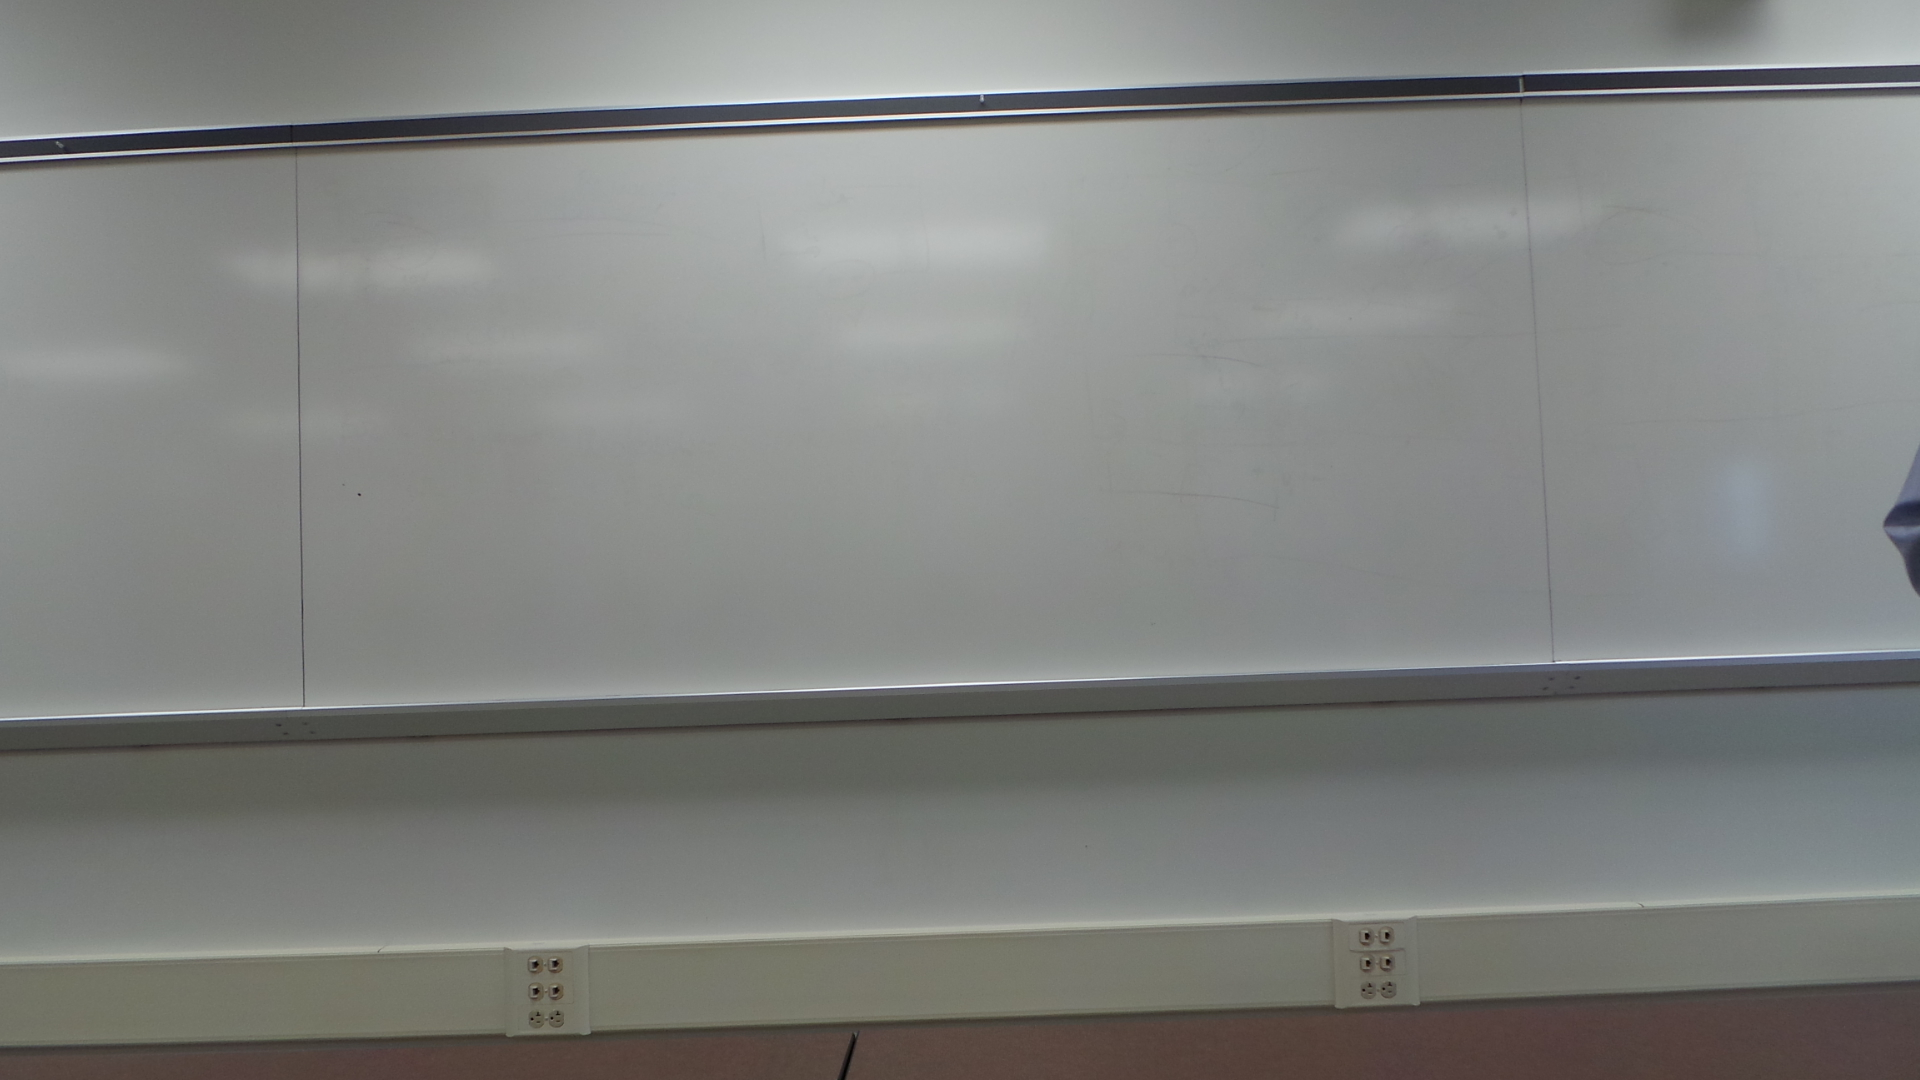
\includegraphics[scale=0.1]{images/colorbalance_1}

\end{figure}
		
\begin{figure}[H]
\centering
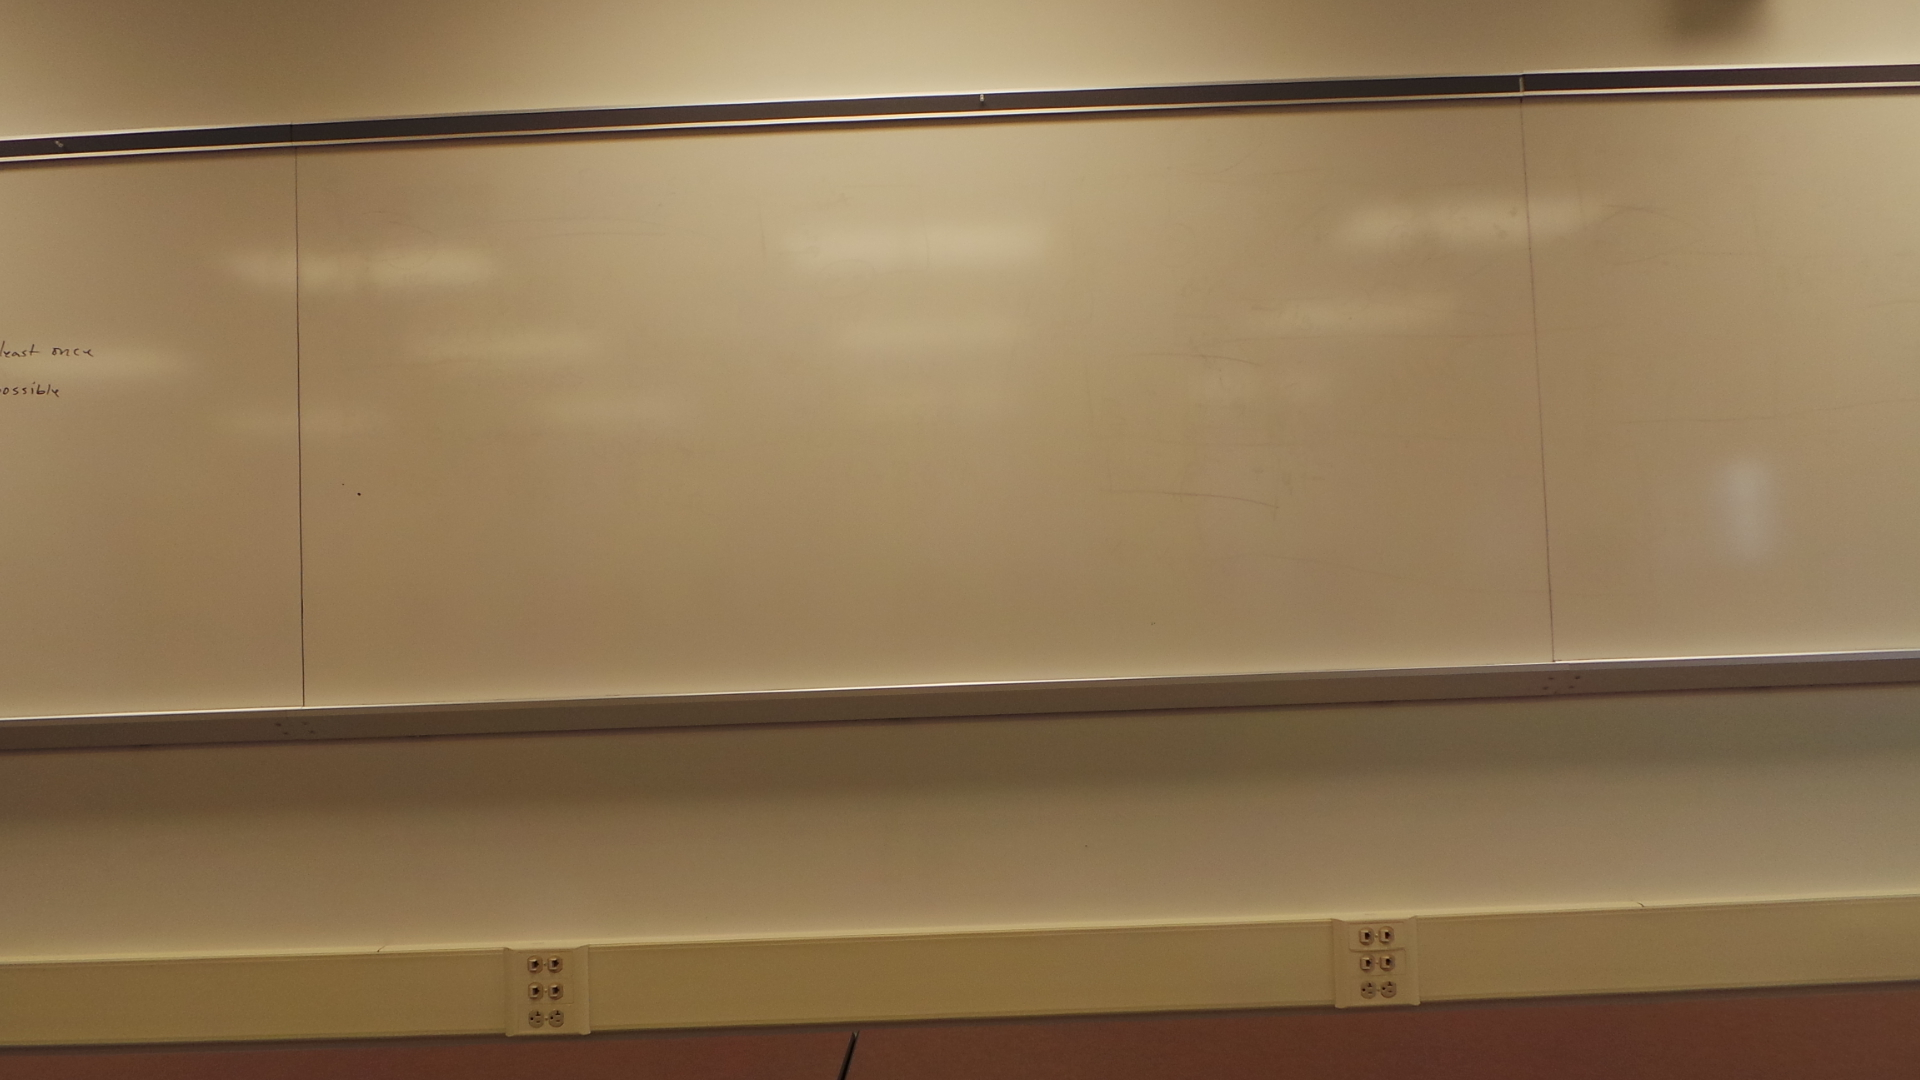
\includegraphics[scale=0.1]{images/colorbalance_2}

\end{figure}	
		
\begin{figure}[H]
\centering
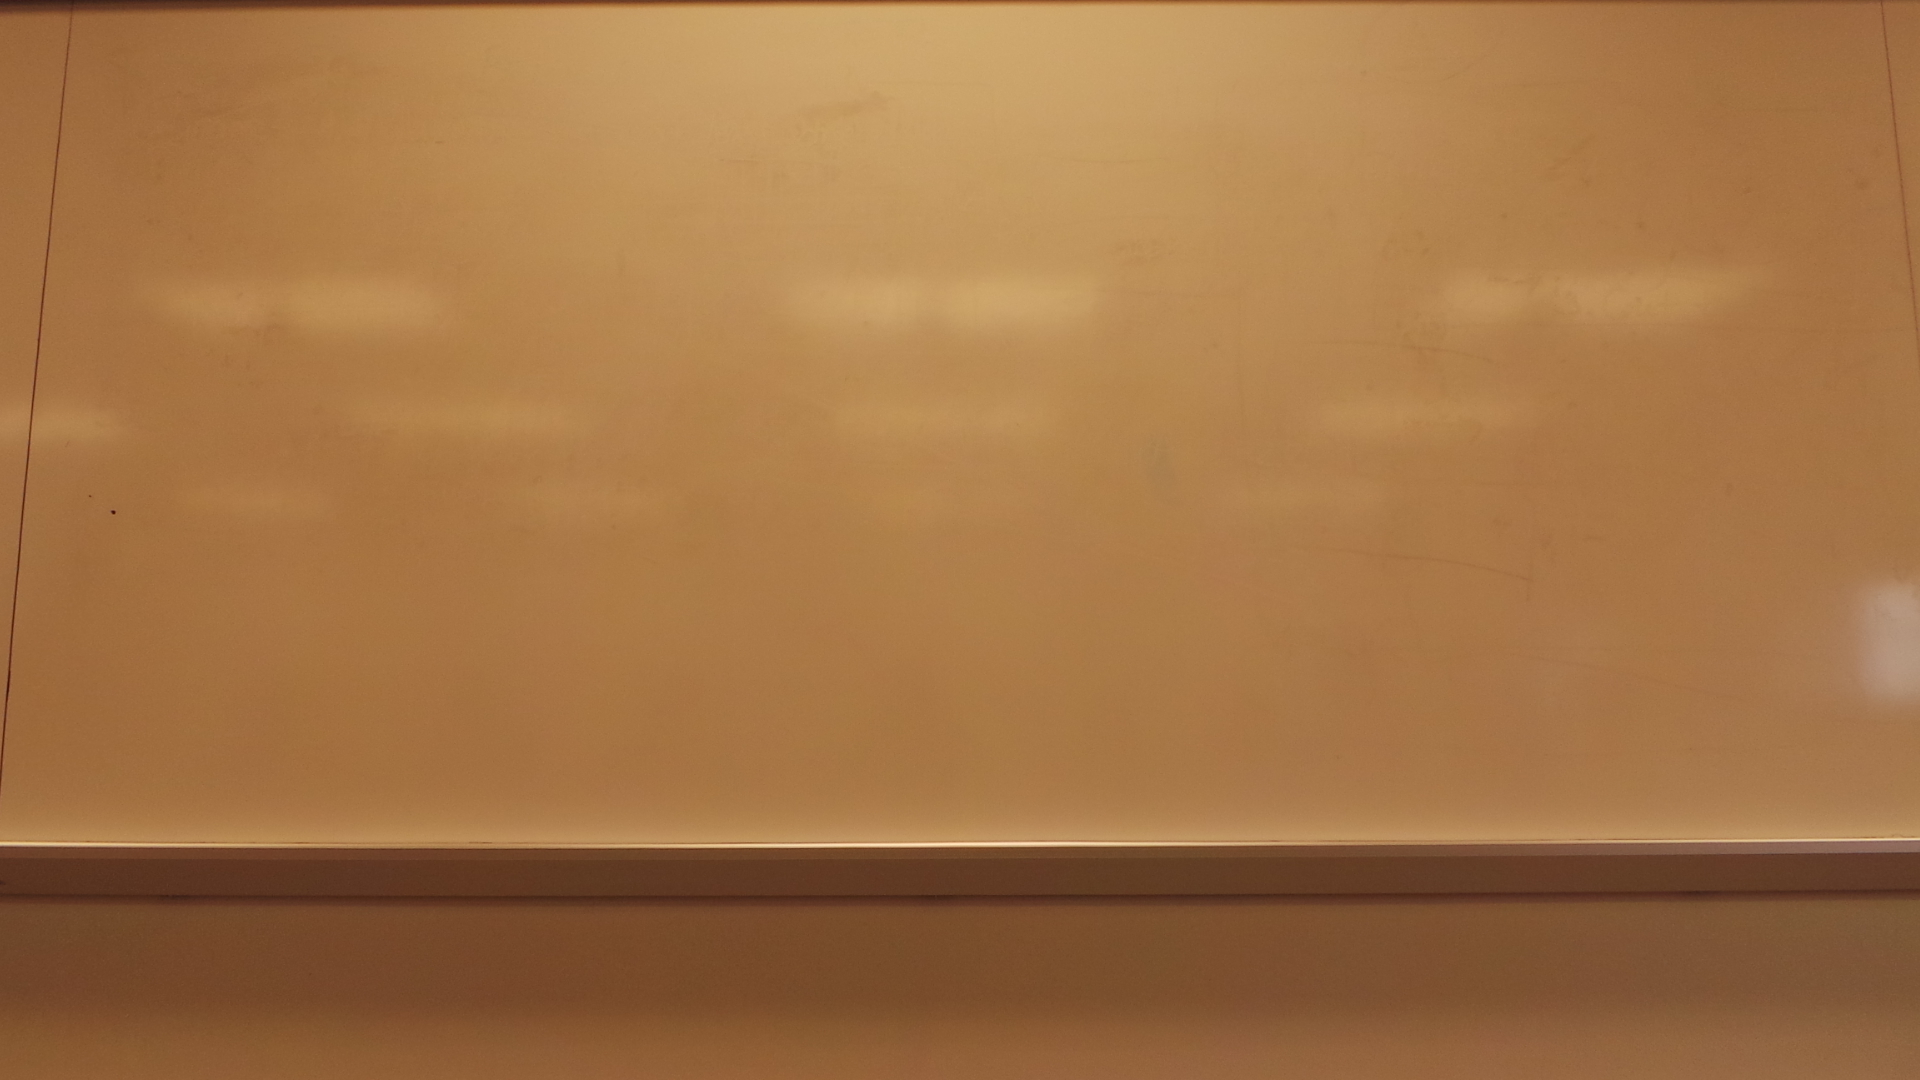
\includegraphics[scale=0.1]{images/colorbalance_3}

\end{figure}		

As a result of this, the analysis system is having trouble classifying cells.  It calculates the whiteboard color based on the average luminance of all of the images, but since the overall shade keeps changing, this average value is not helpful.  As a result, the images that happen to have a similar tone as the calculated average are classified correctly, but images that have much darker or lighter tones are incorrectly classified with massive amounts of foreground objects.  Phil is working on a fix to this, so when we try to get another image set on Friday, this should be fixed.

\begin{figure}[H]
\centering
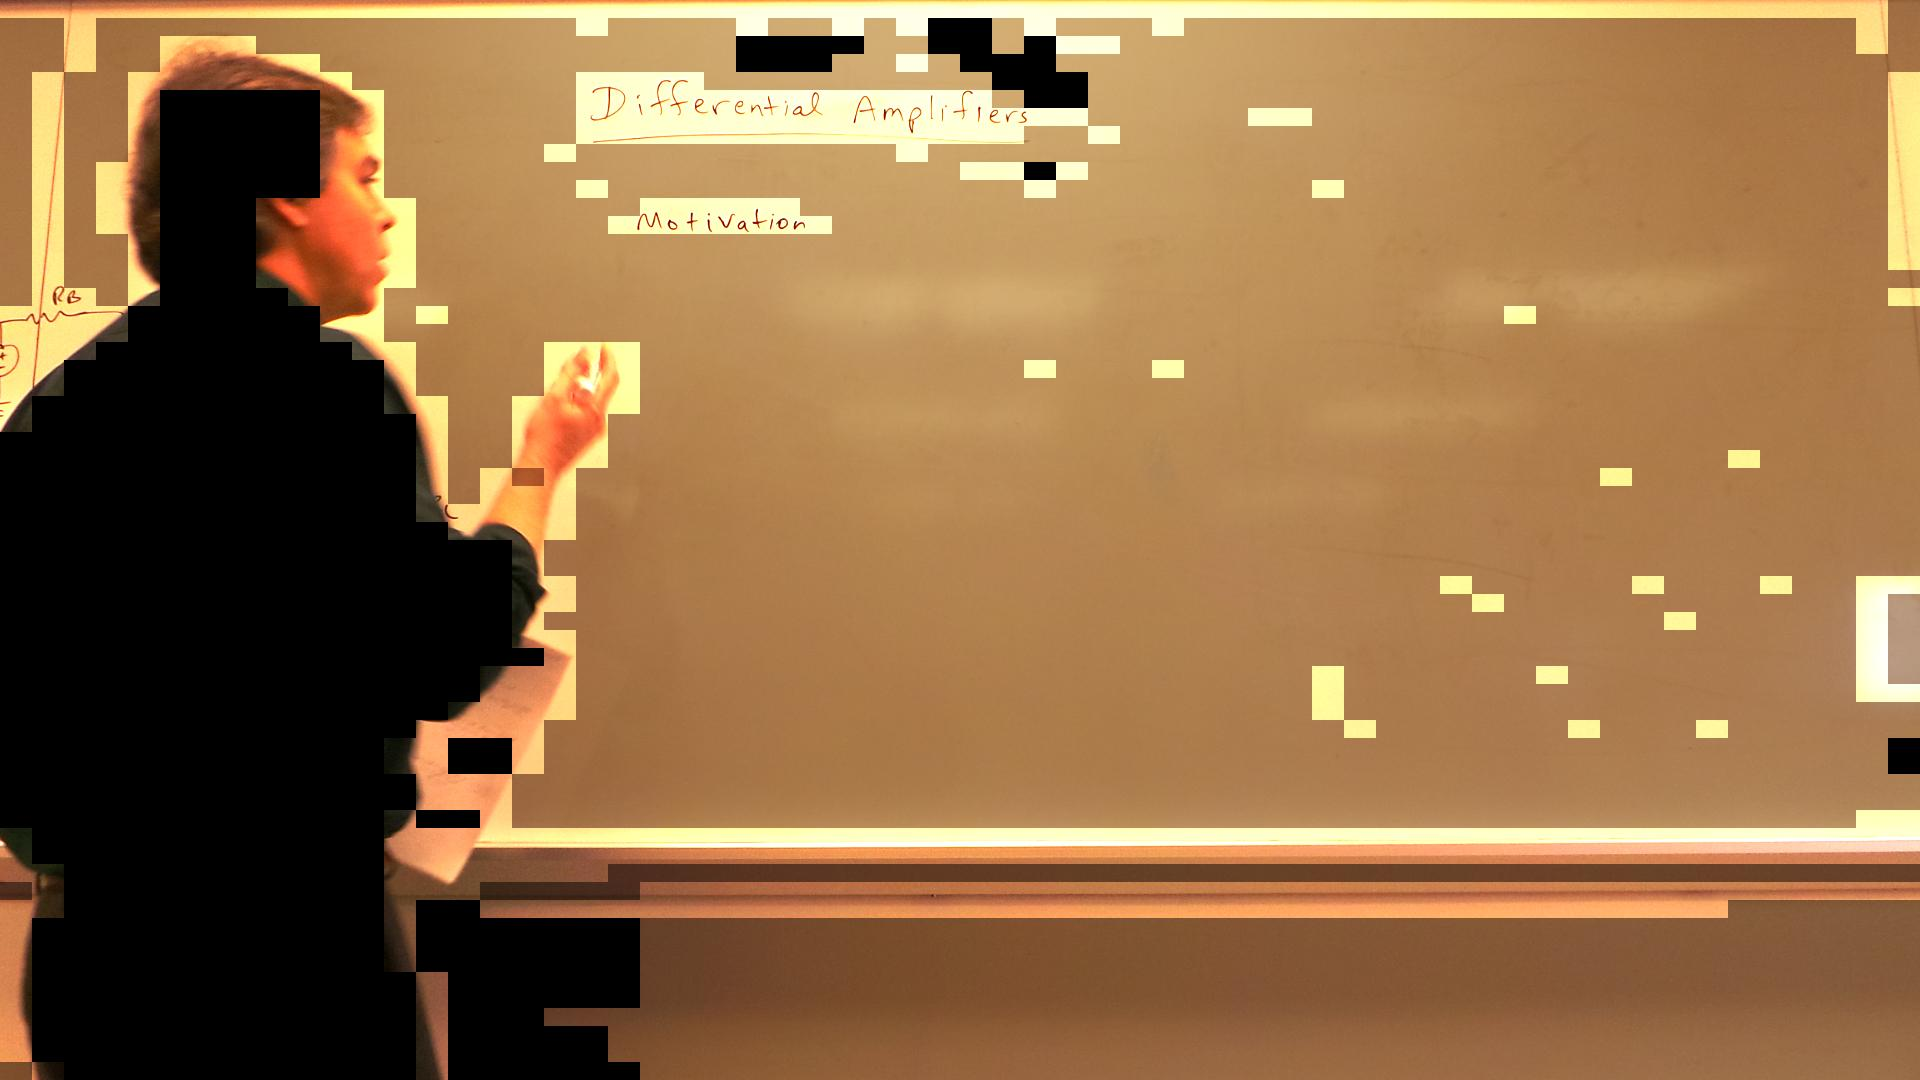
\includegraphics[scale=0.2]{images/badIw_1}
\caption{Image with $I_w$ similar to calculated average}
\end{figure}	
		
\begin{figure}[H]
\centering
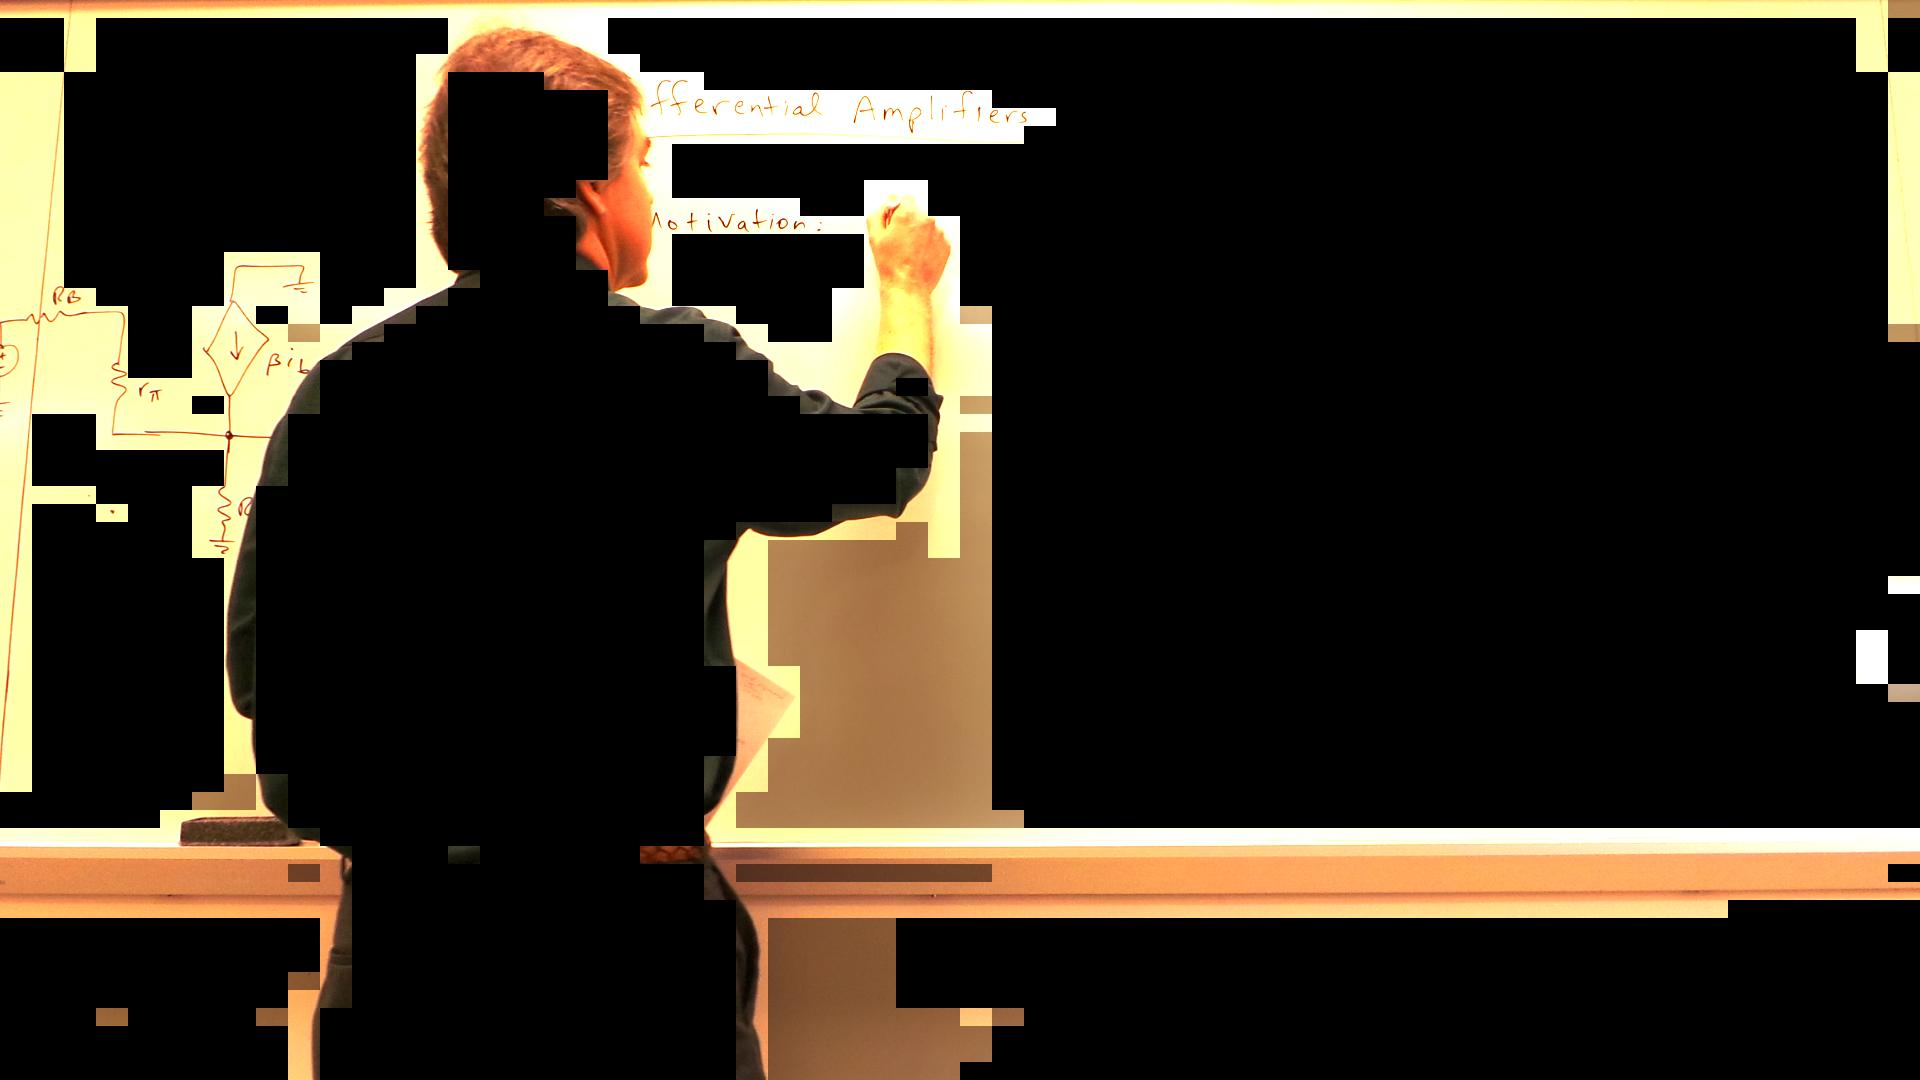
\includegraphics[scale=0.2]{images/badIw_2}
\caption{Image with $I_w$ different from calculated average}
\end{figure}

	\subsection*{Memory Overload}
	I quickly learned that there is no way for us to process the entire almost-700 image set at once.  The program as currently written will use up all of my available memory when trying to run on a set of 50 images (on my Windows laptop).  The Linux OS we use on our dedicated analysis computer will not even let us open 700 images at once!  Our plan now is to break processing up into sets of (hopefully) 50 images.  We also have ideas to bring down memory consumption, including more diligent opening and closing of the JPEG files.



	%Twenty-Third Entry
	\section{Spacial Cell Filtering (1/31/2013)}	
		I'm continuing to work on cell classification.  After the basic classification, the next step that Microsoft follows is to implement spatial and temporal cell filtering, which reclassifies some cells that meet specific criteria.  I implemented part of the spatial filtering in the script.  Now, any foreground cells that are completely surrounded by stroke and/or board cells are converted to stroke cells.  This is because in reality, a foreground cell would never appear completely isolated from other foreground cells.  Changing it to a stroke cell minimizes its negative impact on the image, since it is actually not a foreground object.  
\begin{figure}[H]
\centering
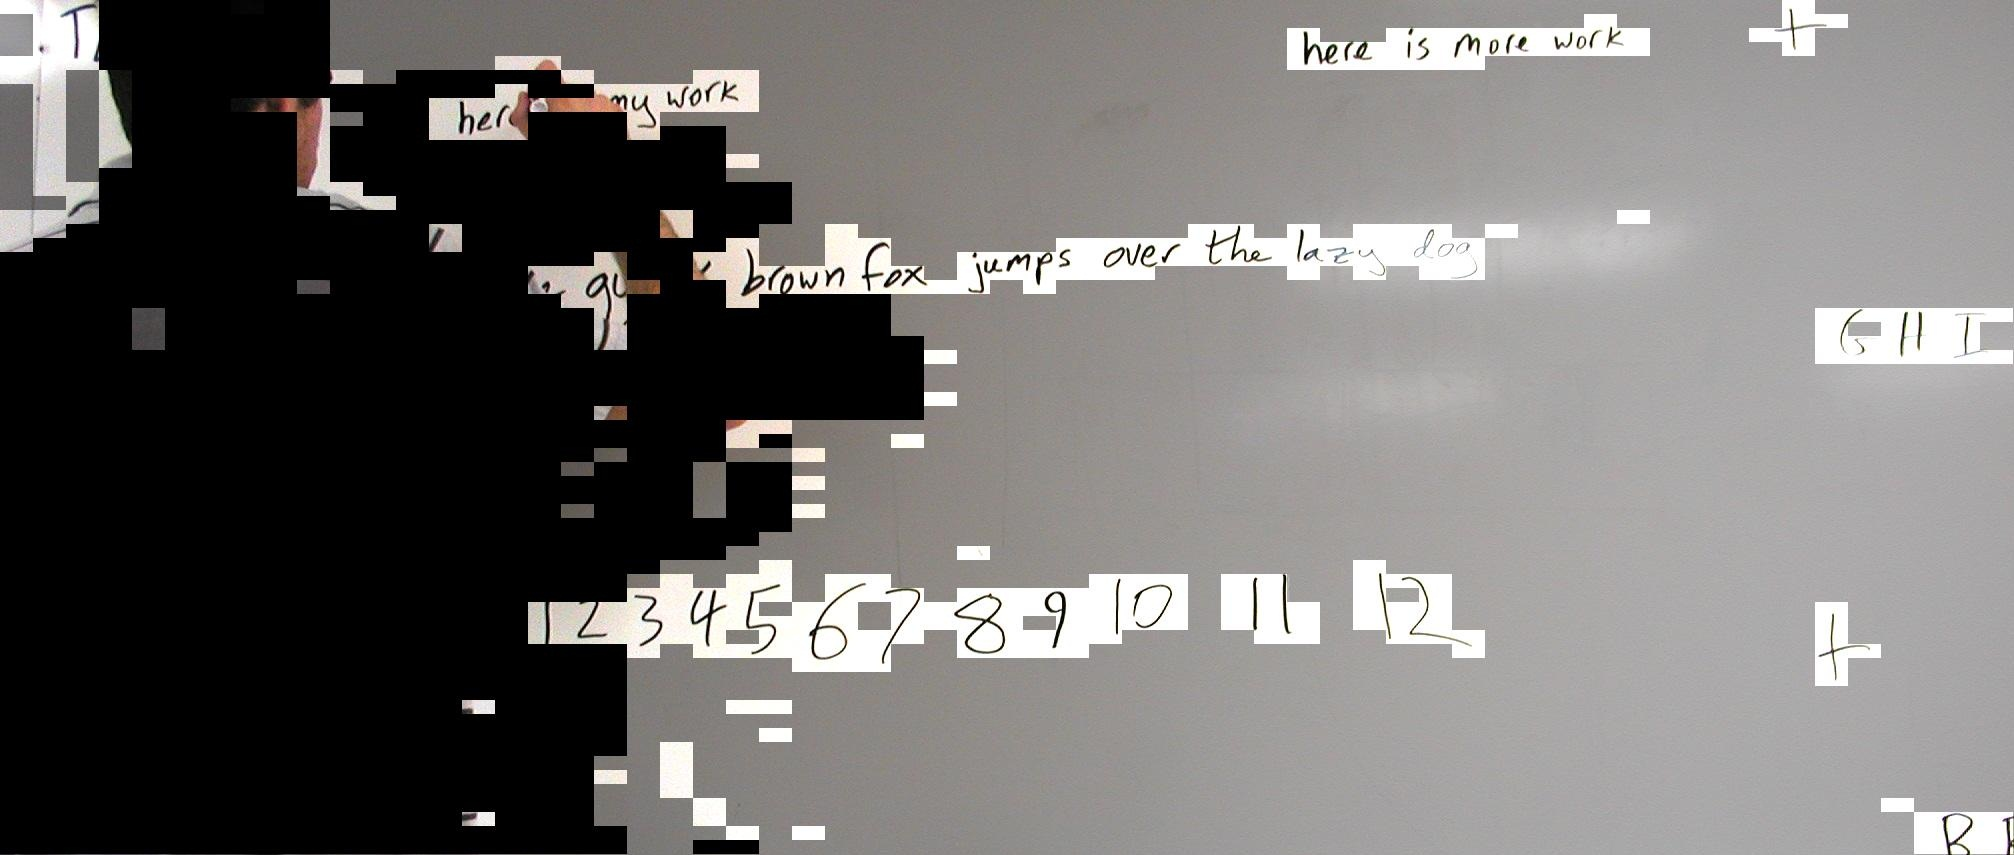
\includegraphics[scale=0.2]{images/afterSpatial1}
\caption{After Partial Spatial Filtering}
\end{figure}
		
\begin{figure}[H]
\centering
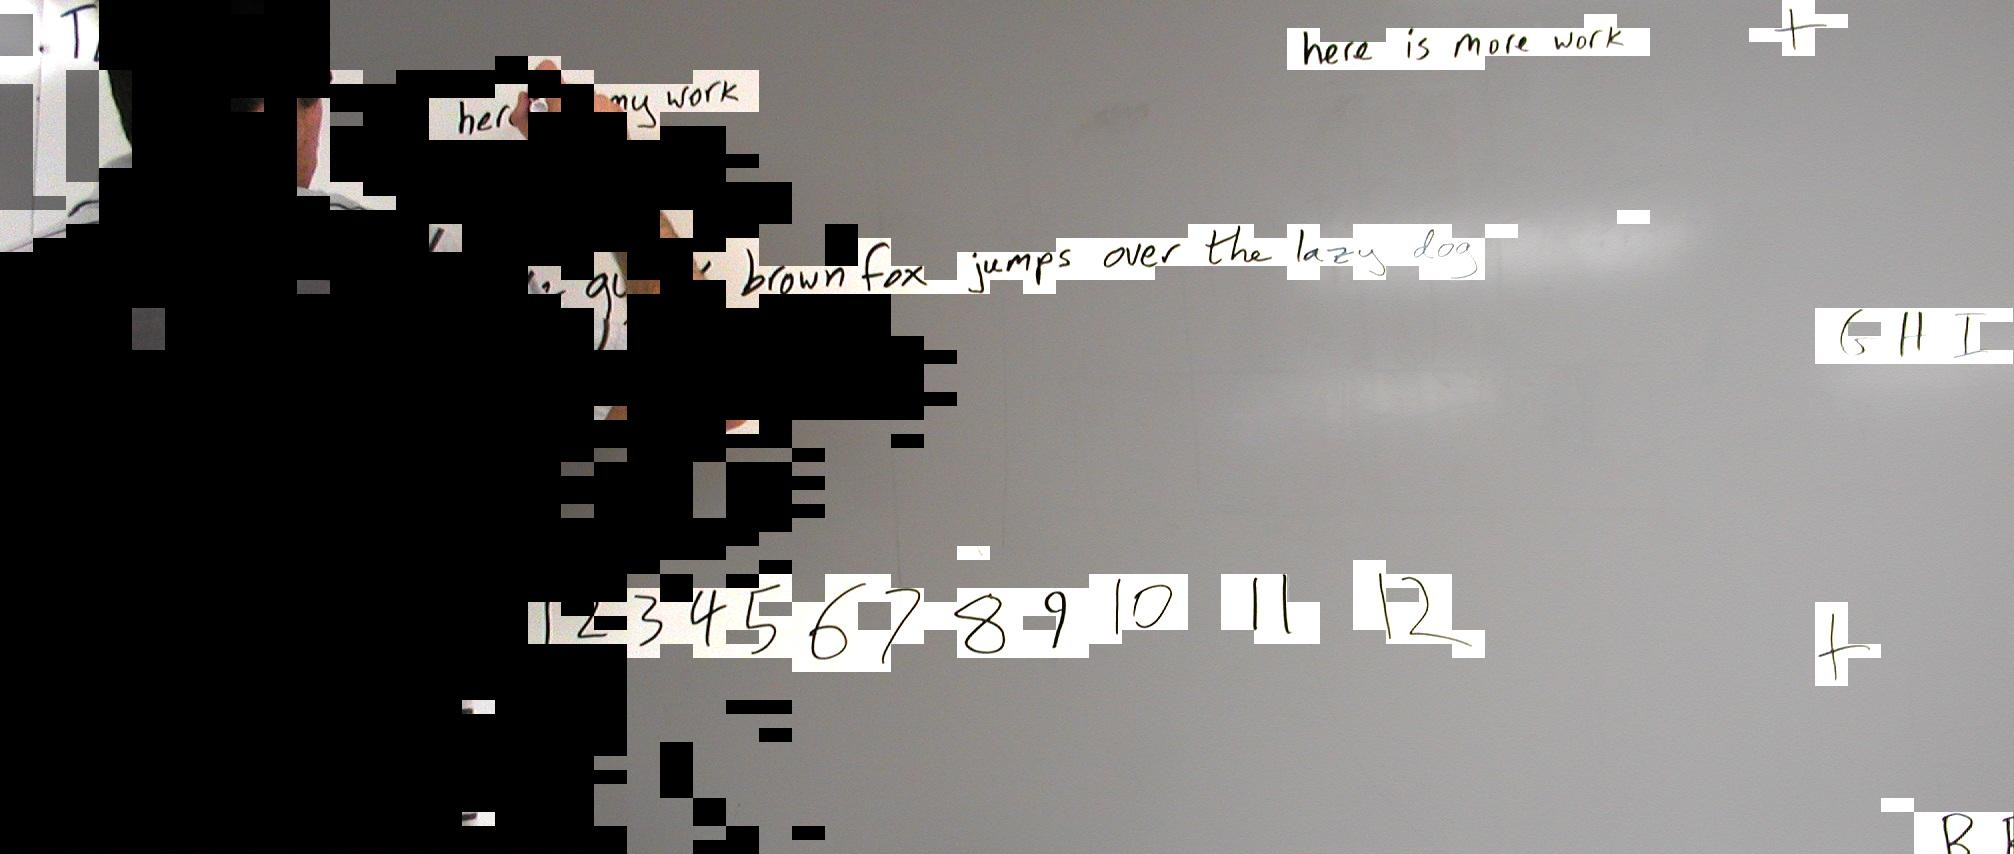
\includegraphics[scale=0.2]{images/beforeSpatial1}
\caption{Before Partial Spatial Filtering}
\end{figure}	
This does not affect a lot of cells, which is good as far as our classification method is concerned.  Next, I will implement more spatial filtering, as well as some temporal filtering, which will further improve our cell classification.
	%Twenty-Second Entry
	\section{Object-Orienting the Code (1/24/2013)}	
		We decided that going forward, we should work in an object-oriented coding environment.  Phil is the most experienced working with O-O code, so he is writing the bulk of the program.  I am converting the math that I wrote for cell classification into an O-O format.  Since the separate now divide the image into physical cells and process the images inside those cells, the variables in my code no longer have to be two- and three-dimensional because they are no longer in nested for-loops.  For instance, instead of the statement:
\begin{verbatim}
 if abs(I[i][j][k][0]-Iw[i][j][0][0])/(sig[i][j][k][0]+sigw) < Tw and sig[i][j][k][0]/sigw < Tsig:
\end{verbatim}
It now looks like:
\begin{verbatim}
if abs(I-Iw)/(sig+sigw) < Tw and sig/sigw < Tsig:
\end{verbatim}
This line alone is almost enough to show how much easier to read object oriented code can be.  
\\
One remaining problem is that for the variable $I_w$ in the above calculations (which represents the luminance of a cell of the whiteboard over time), we need access to all of the cells over time, and as the code is currently written, we don't have a way to do that easily. Phil is looking into solving this.
	
	%Twenty-First Entry
	\section{Camera Selection Decision Matrix ()1/21/2013}
		With less than a month until Panel 4, we are running out of time to get a camera for our project.  We have been set on the Samsung Galaxy Camera for some time, but we needed to show our decision process better to justify the decision.  I am making a set of decision matrices that compare and contrast various camera options to determine which device will work best with the ProPANE system.  I am comparing many aspects, including battery life, zoom, resolution, price, and many others.  It is completely objective.  That being said, we believe that the best option is still the Galaxy Camera, and this analysis should show that convincingly.
	
	%Twentieth Entry
	\section{Even More Cell Classification Over Time (11/30/2012)}
		I decided to try processing the image using the same as in the previous entry, except using the whiteboard color calculated from one empty board picture, instead of the one calculated from the sequence of images.  In the future, once we implement some of the error corrections that Microsoft used, we shouldn't get the weird anomalies in the whiteboard color that we're getting now.  However, for now I wanted to see what this gave me.  The results were interesting.  \\
		 	
		 	I used the single image whiteboard color calculation instead of the sequential one (see the second and third images in my previous worklog entry).  Here is a comparison of the cell classification from each method:
		 	
\begin{figure}[H]
\centering
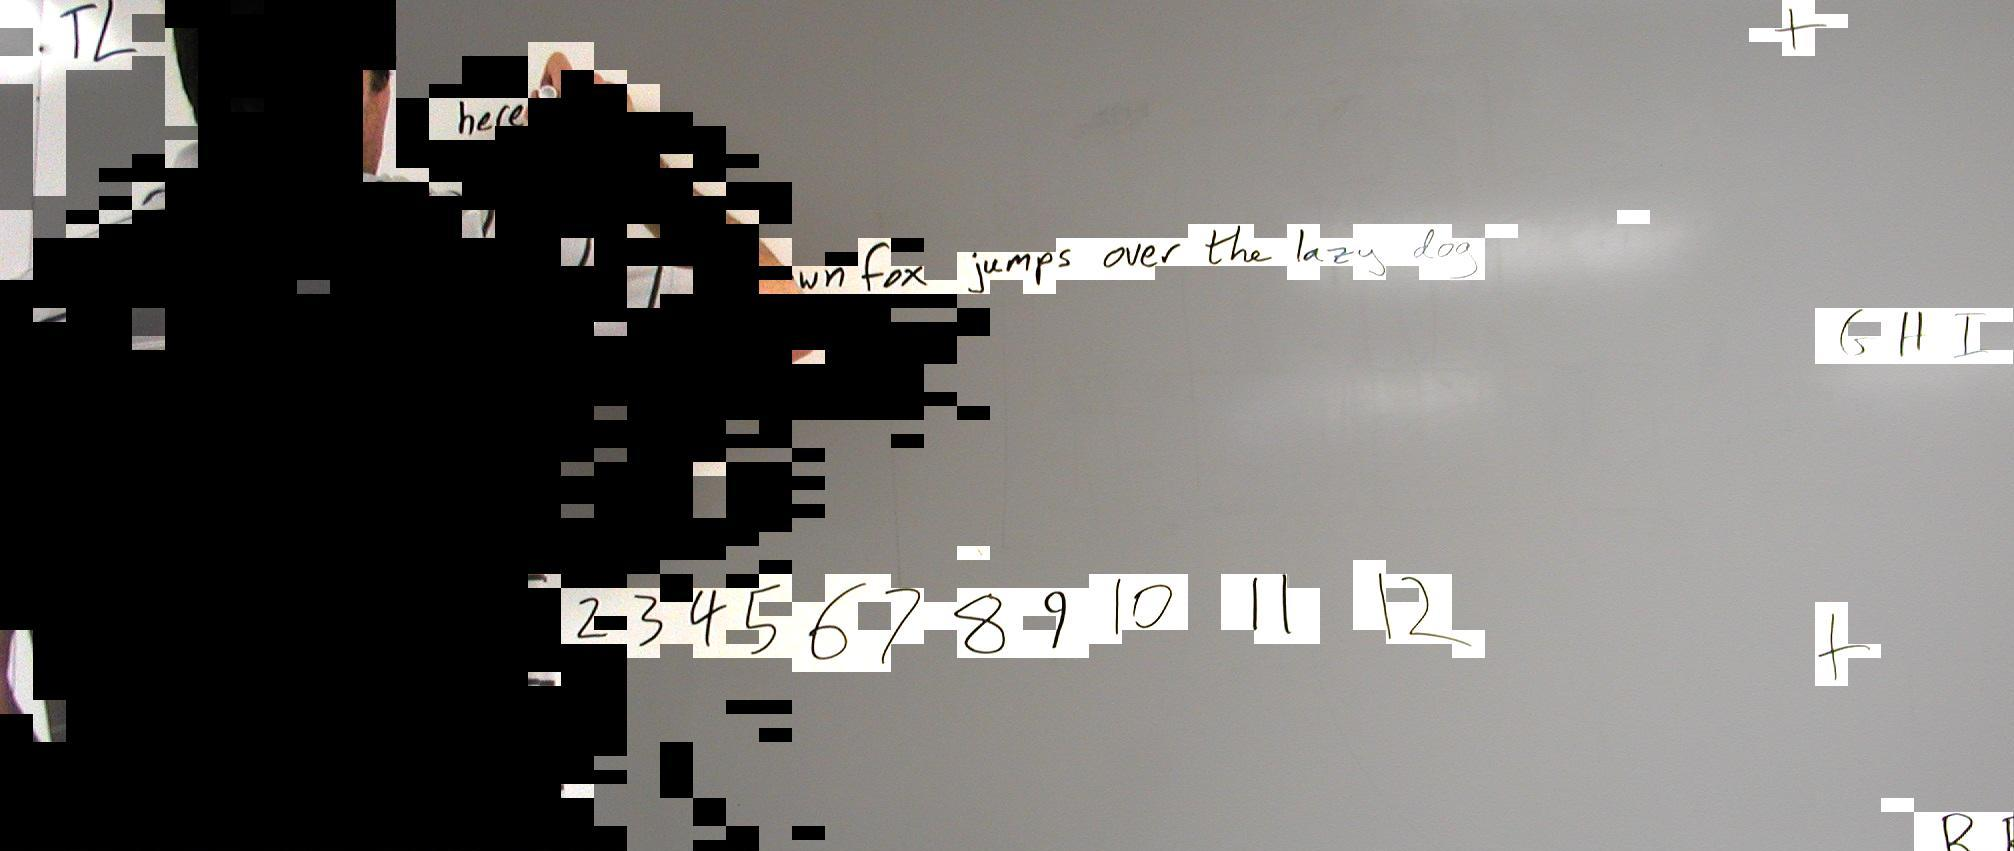
\includegraphics[scale=0.25]{images/griffin_foreground1}
\caption{Sequence of images}
\end{figure}
		
\begin{figure}[H]
\centering
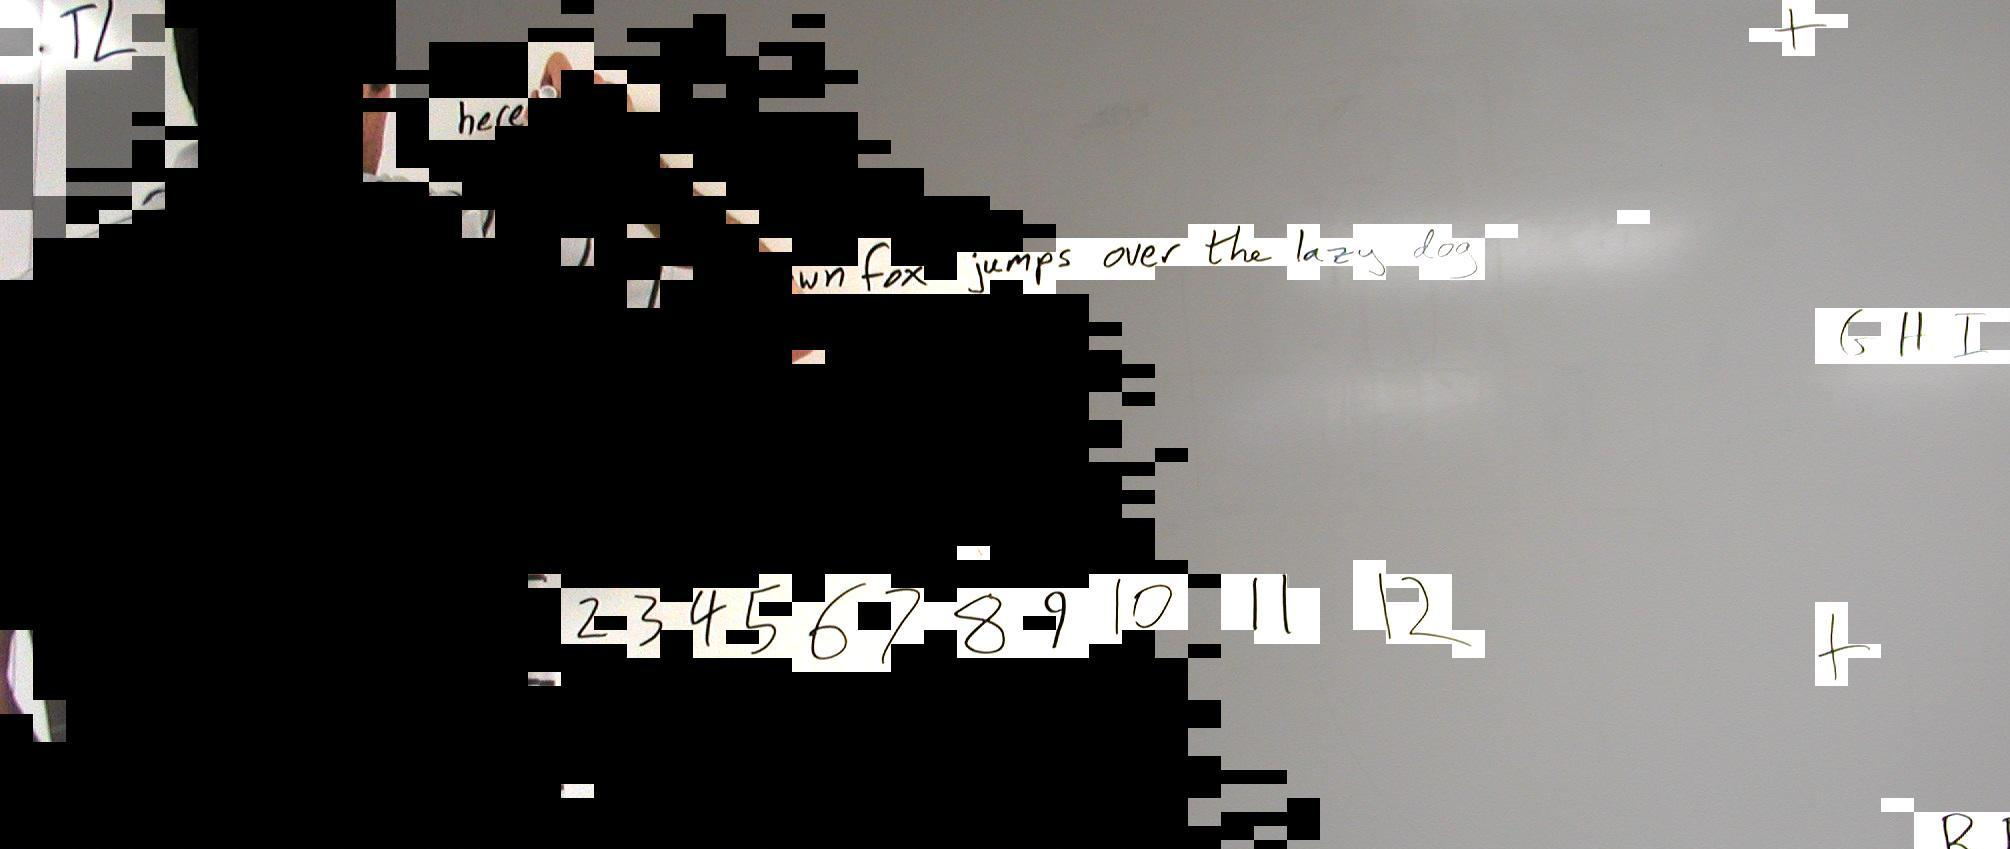
\includegraphics[scale=0.25]{images/griffin_foreground2}
\caption{Single image}
\end{figure}	
	
	The stroke detection is essentially identical in both images, but the foreground/whiteboard cell detection varies quite a bit.  For some reason, the single image whiteboard test thinks that many cells with nothing in them contain foreground objects.
	
\begin{figure}[H]
\centering
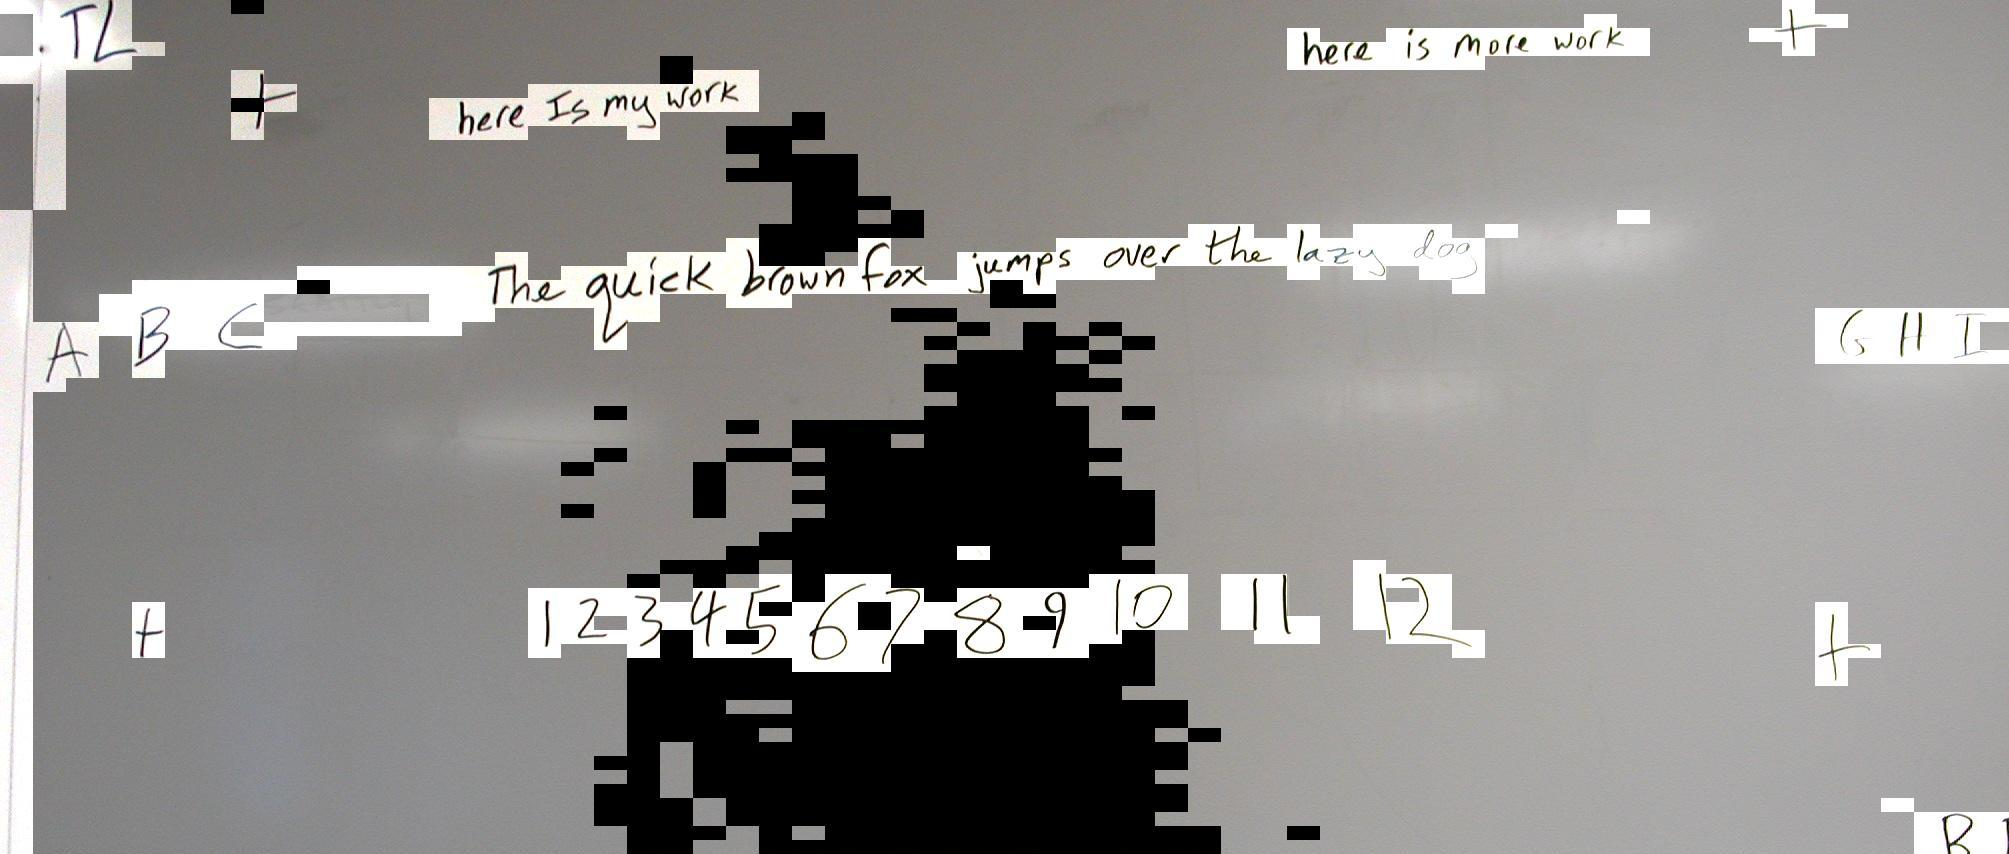
\includegraphics[scale=0.25]{images/emptyboard_overtime}
\caption{Sequence of images}
\end{figure}
		
\begin{figure}[H]
\centering
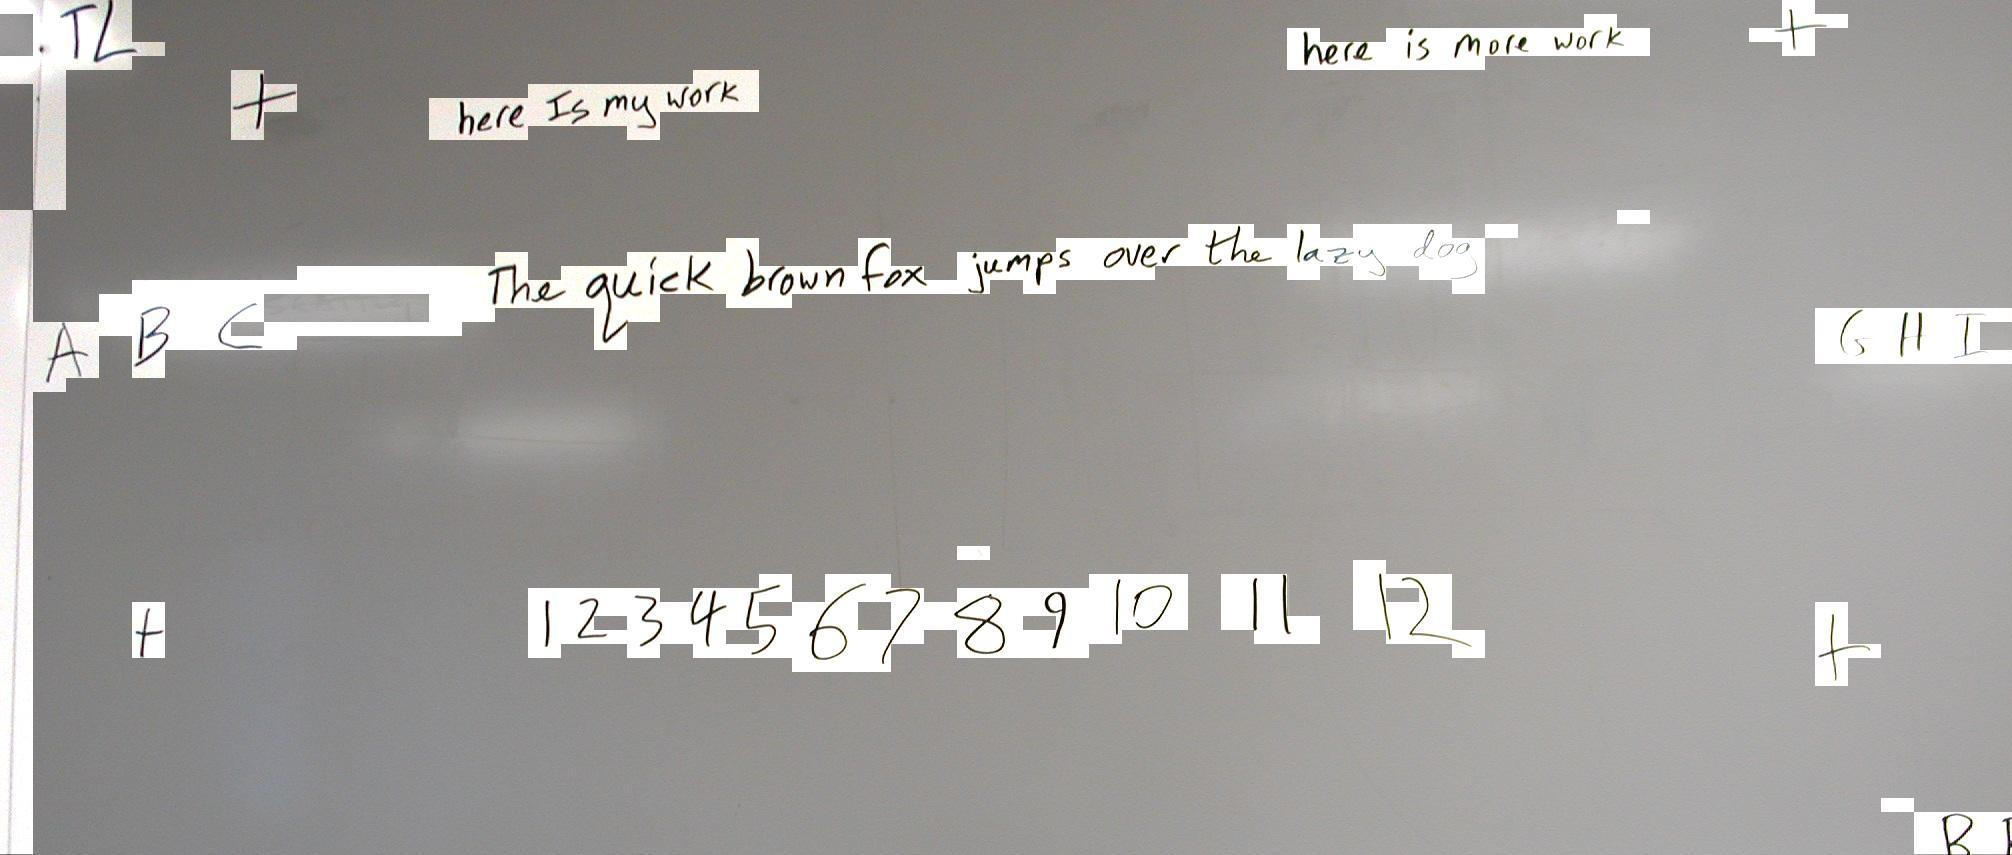
\includegraphics[scale=0.25]{images/emptyboard_single}
\caption{Single image}
\end{figure}

These are the processed images of the last image in the set, which is an unobstructed view of the board.  Again, stroke cell detection is identical.  However, the single image whiteboard color test correctly determines that there are no foreground cells, while the sequence of images whiteboard color test believes that there is a foreground object.  This is due to the aforementioned anomalies in the whiteboard color detection due to the small image set, and I believe that it will go away as our testbed is expanded.  For reference, look at the whiteboard image from the sequence of images.  The visible anomalies are clearly in the same locations as the erroneously detected foreground cells.

\begin{figure}[H]
\centering

\includegraphics[scale=0.25]{images/background_overtime}
\caption{The image of the whiteboard color as detected over the whole sequence}
\end{figure}	
	%Ninteenth Entry
	\section{More Cell Classification Over Time (11/27/2012)}
		I implemented numpy to calculate the mean and standard deviation of the whiteboard cells over time.  The idea is similar to before, but I think that earlier I was calculating it wrong.  This did not immediately fix the problem.  However, I did find the solution.  Even with the whiteboard cells having a very small standard deviation, the standard deviation of the stroke cells were all over the place.  Instead of using the value of $Tsig = 2$ as in Microsoft's paper, I looked at some of the values that I was getting and decided to try some higher values of $Tsig$.    This drastically improved the processing of the images.  Now, cell classification works for all three types of cell.  \\
		
		One interesting result of these changes is that the whiteboard color used for calculations looks good in most areas, but there are unusually dark patches in a couple places which throw off the uniformity of the board color.  I think that this is due to using a relatively small image set at the moment, so the person in the foreground is in certain spots for a much greater percentage of the time than they would normally be.

\begin{figure}[H]
\centering
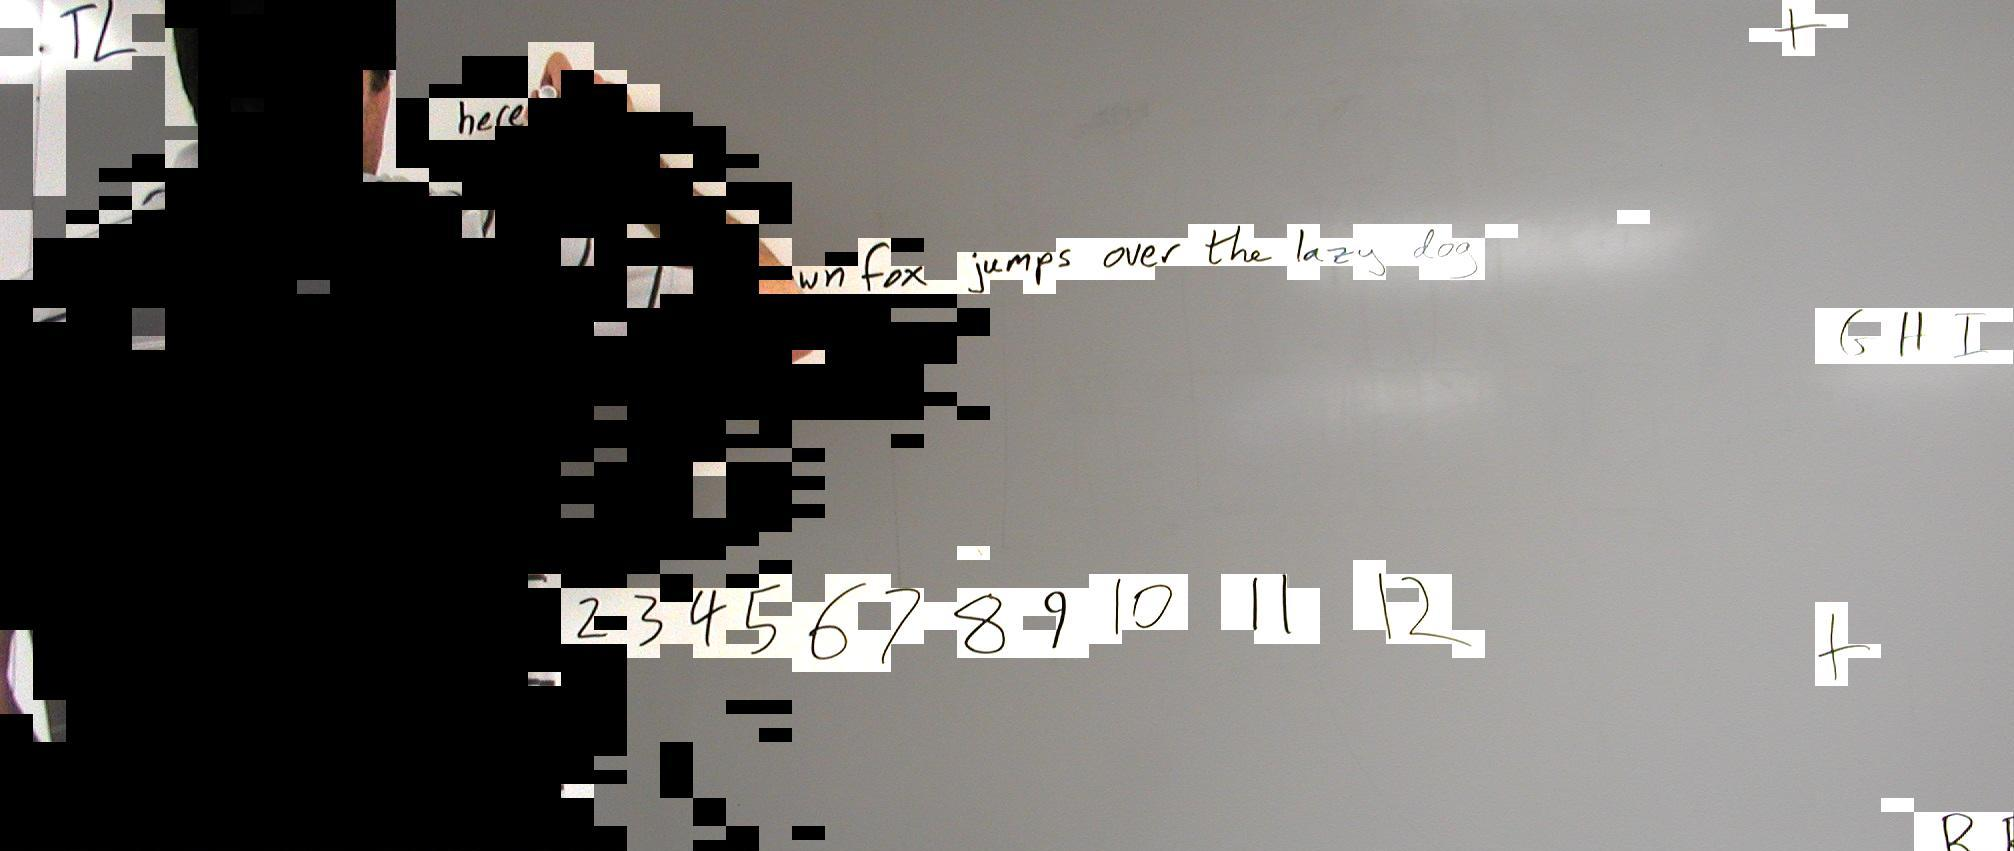
\includegraphics[scale=0.25]{images/griffin_foreground1}
\caption{first image in sequence, processed, using Tsig = 40.  Clear foreground, stroke, and whiteboard cell detection}
\end{figure}
		
\begin{figure}[H]
\centering

\includegraphics[scale=0.25]{images/background_overtime}
\caption{The image of the whiteboard color as detected over the whole sequence}
\end{figure}	

\begin{figure}[H]
\centering

\includegraphics[scale=0.2]{images/whiteboard_single}
\caption{The image of the whiteboard color as detected from one image of a whiteboard with no foreground objects}
\end{figure}		
	%Eighteenth Entry 
	\section{Cell Classification Over Time (11/19/2012)}
		I reworked the code I wrote for cell classification to work on a sequence of images over time.  Now, instead of an image cell being defined as cell\_image[$i$][$j$] (where $i$ and $j$ are width and height dimensions), they are defined as cell\_image[$i$][$j$][$k$], where $k$ is the index of the cell in the sequence of images.  That is, each cell\_image[$i$][$j$] comes from a different image $k$.  \\ 
		
		Now that the code is working with a sequence of images, it can detect foreground objects, since their detection requires an unusual change over time of individual cells.  However, a strange problem that I'm encountering now is that the program now seems to think that every non-foreground cell is a stroke cell.  I think it has to do with how the color of the whiteboard is calculated. I'm looking at another way to do some math on it... I think the \href{http://numpy.scipy.org/}{numpy} math library for Python will be very helpful for this. 
		
\begin{figure}[H]
\centering
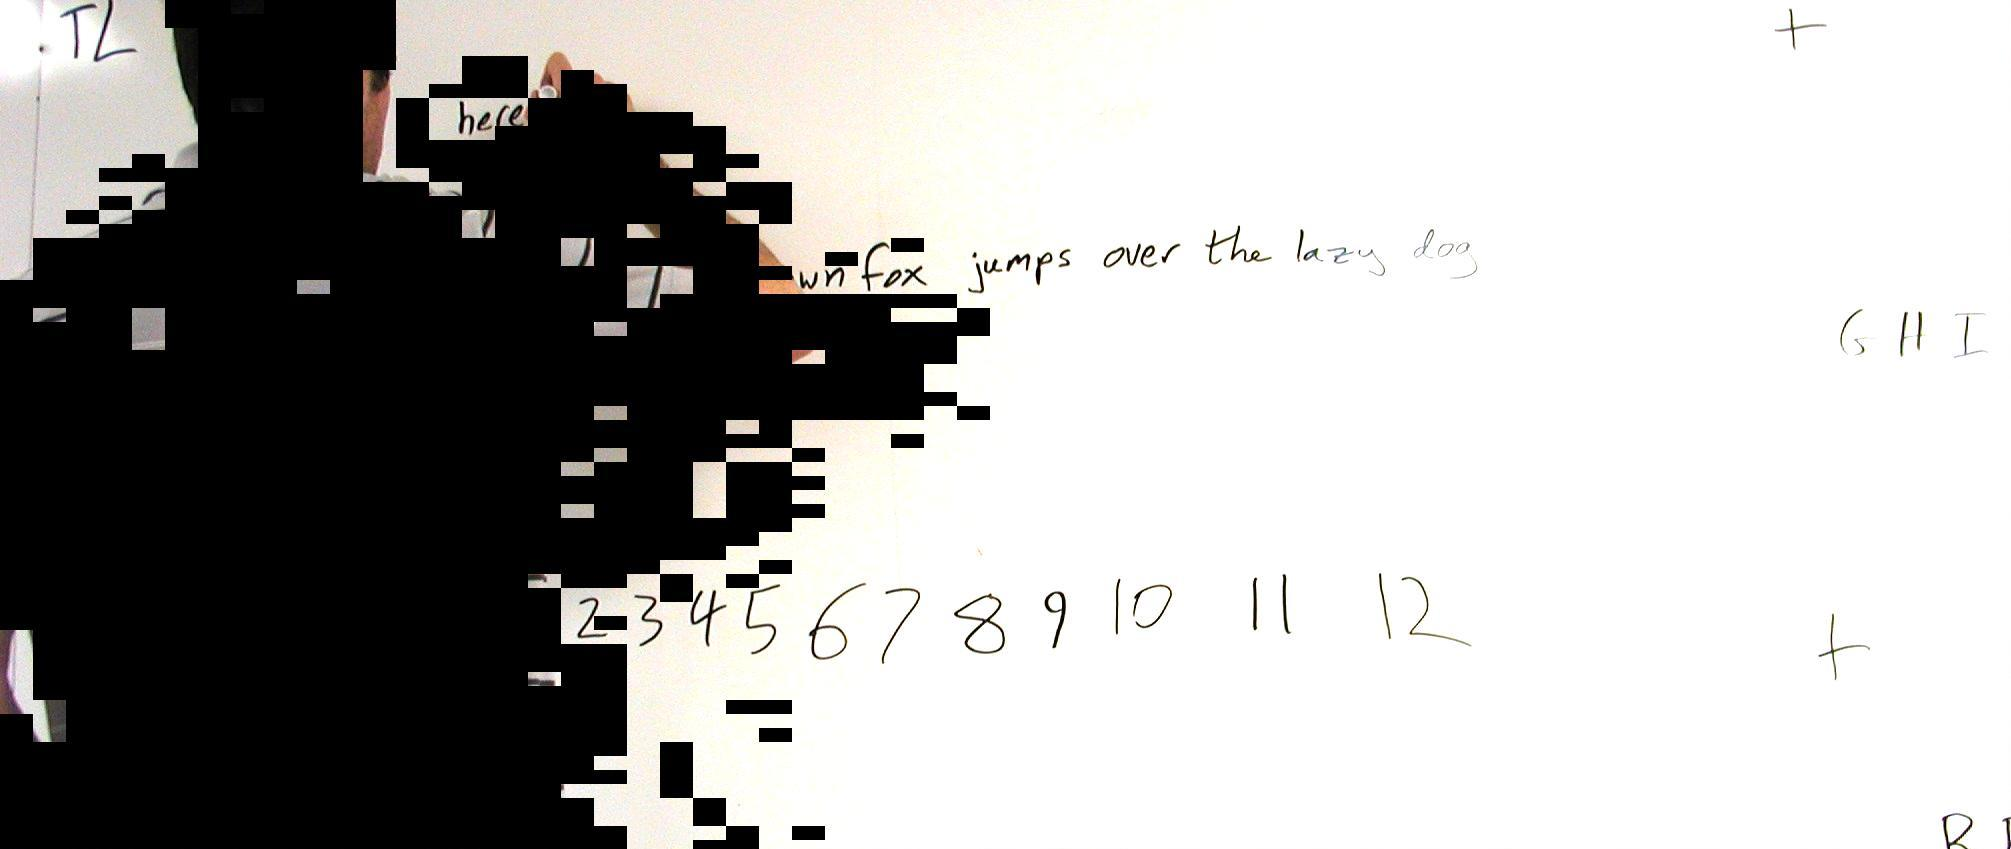
\includegraphics[scale=0.3]{images/allstrokecells}
\caption{first image in sequence, processed. Note foreground cell detection and lack of whiteboard detection (brightness indicates stroke cell detection)}
\end{figure}
		
		Clearly, the foreground detection is not perfect either, but without any of the error correction methods implemented by Microsoft, I think it is a good start.
	%Seventeenth Entry
	\section{Cell Classification (11/14/2012)}
		I continued following Microsoft's image processing algorithm by trying to classify image cells as whiteboard, stroke, or foreground cells.  This is done by calculating the whiteboard color and standard deviation of the whiteboard color, as well as the mean and standard deviation of the current cell color, and using the following comparisons: \\ \\
	 The cell image is classified as a whiteboard cell if and only if \[ {|\bar{I} - \bar{I}_w| \over (\sigma + \sigma_w)}<T_w \quad \textrm{ and } \quad  {\sigma \over \sigma_w }< T_\sigma \] 
and as a stroke cell if and only if
\[{|\bar{I}-\bar{I}_w| \over (\sigma + \sigma_w)}<T_w \quad \textrm{ and } \quad {\sigma \over \sigma_w} \geq T_\sigma \] 
Otherwise, it's classified as a foreground object cell.  In the WCS implementation, $T_w=2$ and $T_\sigma=2$.	

I came up with some python code to accomplish this, which builds on previously written code.  Important to note is that all images we use are in RGB format, meaning they have three color bands.  Currently, I'm doing all calculations by first converting to greyscale images and then processing them.  This could be responsible for some of the errors I'm getting (it probably is) but it was easier for a first proof of concept.  

\begin{verbatim}

Tw = 2
Tsig = 2
bwim = im.convert("L")
sigw = 8
for  i in nsize:
        for j in nsize:
           
            cell_bwimage[i][j] = bwim.crop(cell[i][j])
            Iw[i][j] = white[i][j]            
            I[i][j] = ImageStat.Stat(cell_bwimage[i][j]).mean
            sig[i][j] = ImageStat.Stat(cell_bwimage[i][j]).stddev
          
            if abs(I[i][j][0]-Iw[i][j])/(sig[i][j][0]+sigw) < Tw and sig[i][j][0]/sigw < Tsig:
               cell_id[i][j] = "whiteboard cell"

            elif abs(I[i][j][0]-Iw[i][j])/(sig[i][j][0]+sigw) < Tw and sig[i][j][0]/sigw >= Tsig:
               cell_id[i][j] = "stroke cell"
               temp = ImageEnhance.Brightness(cell_image[i][j])
               temp = temp.enhance(2.0)
               im.paste(temp, cell[i][j])

            else:
               cell_id[i][j] = "foreground object"
               temp = ImageEnhance.Brightness(cell_image[i][j])
               temp = temp.enhance(0)
               im.paste(temp, cell[i][j])
\end{verbatim}

Currently, it will make detected stroke cells brighter for ease of detection, and make foreground cells completely black.  Here are some example output images:


\begin{figure}[H]
\centering
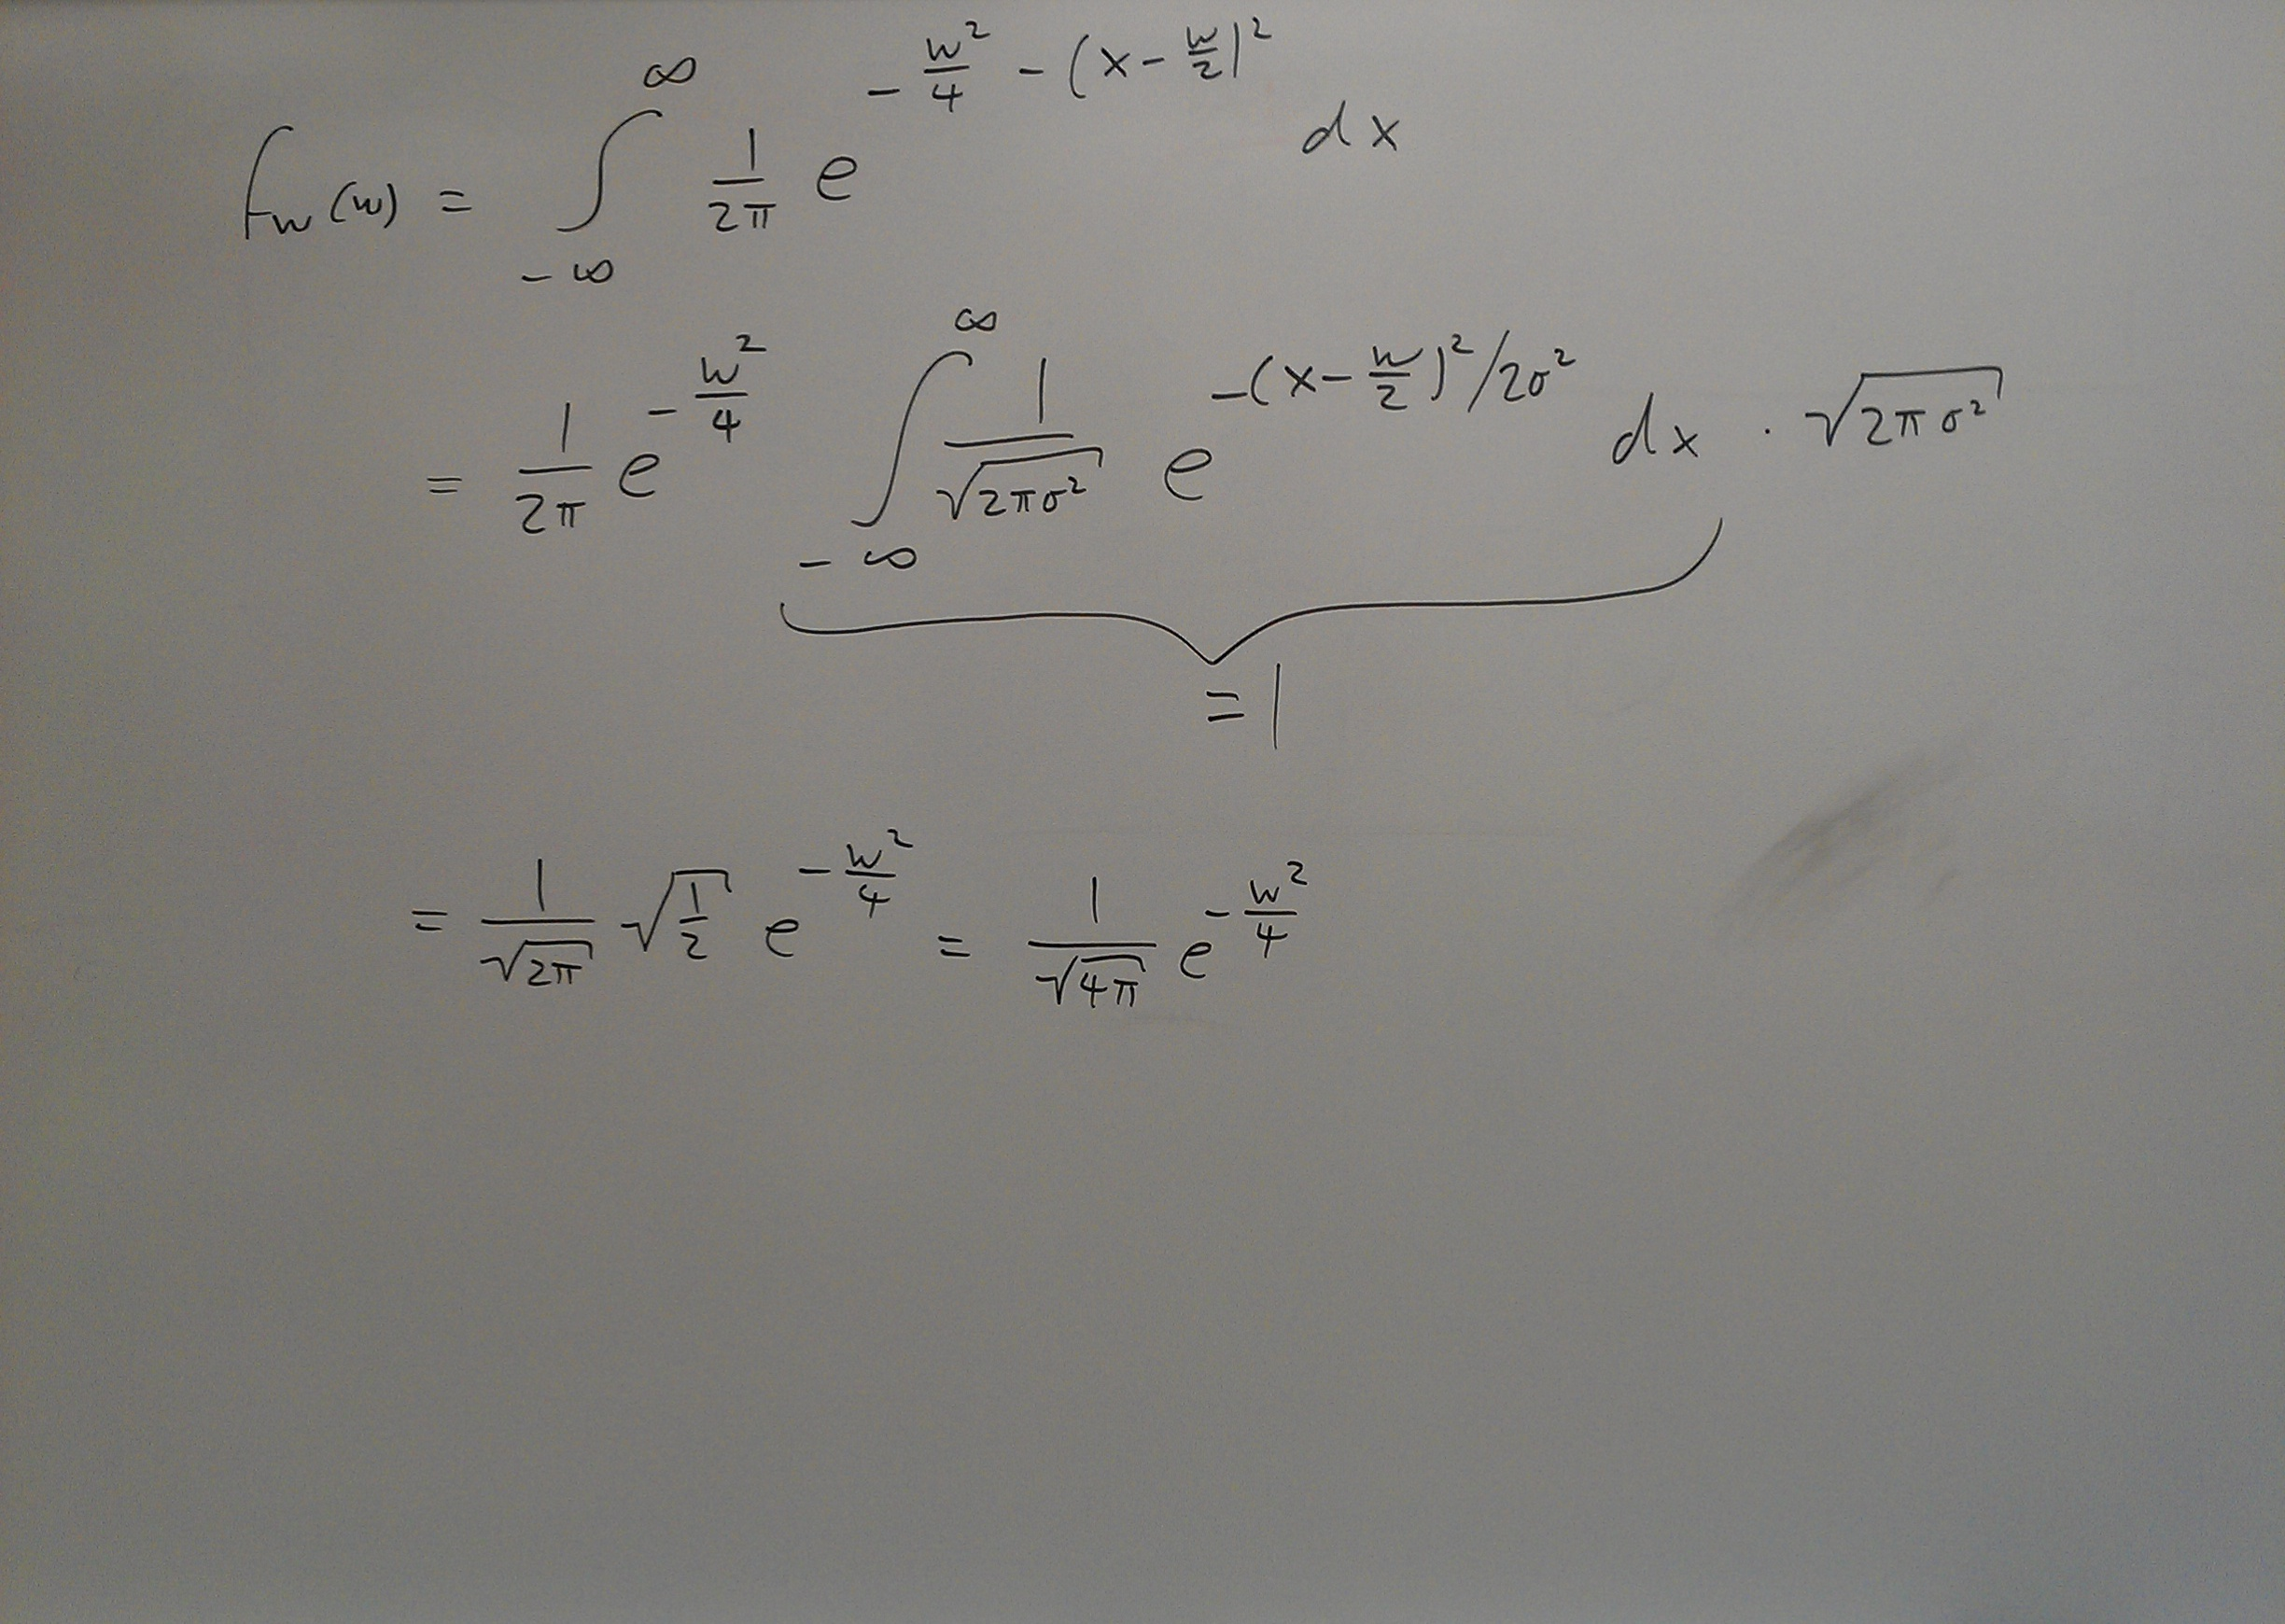
\includegraphics[scale=0.15]{images/wb_nickel_7_crop}
\caption{Unaltered image}
\end{figure}

\begin{figure}[H]
\centering
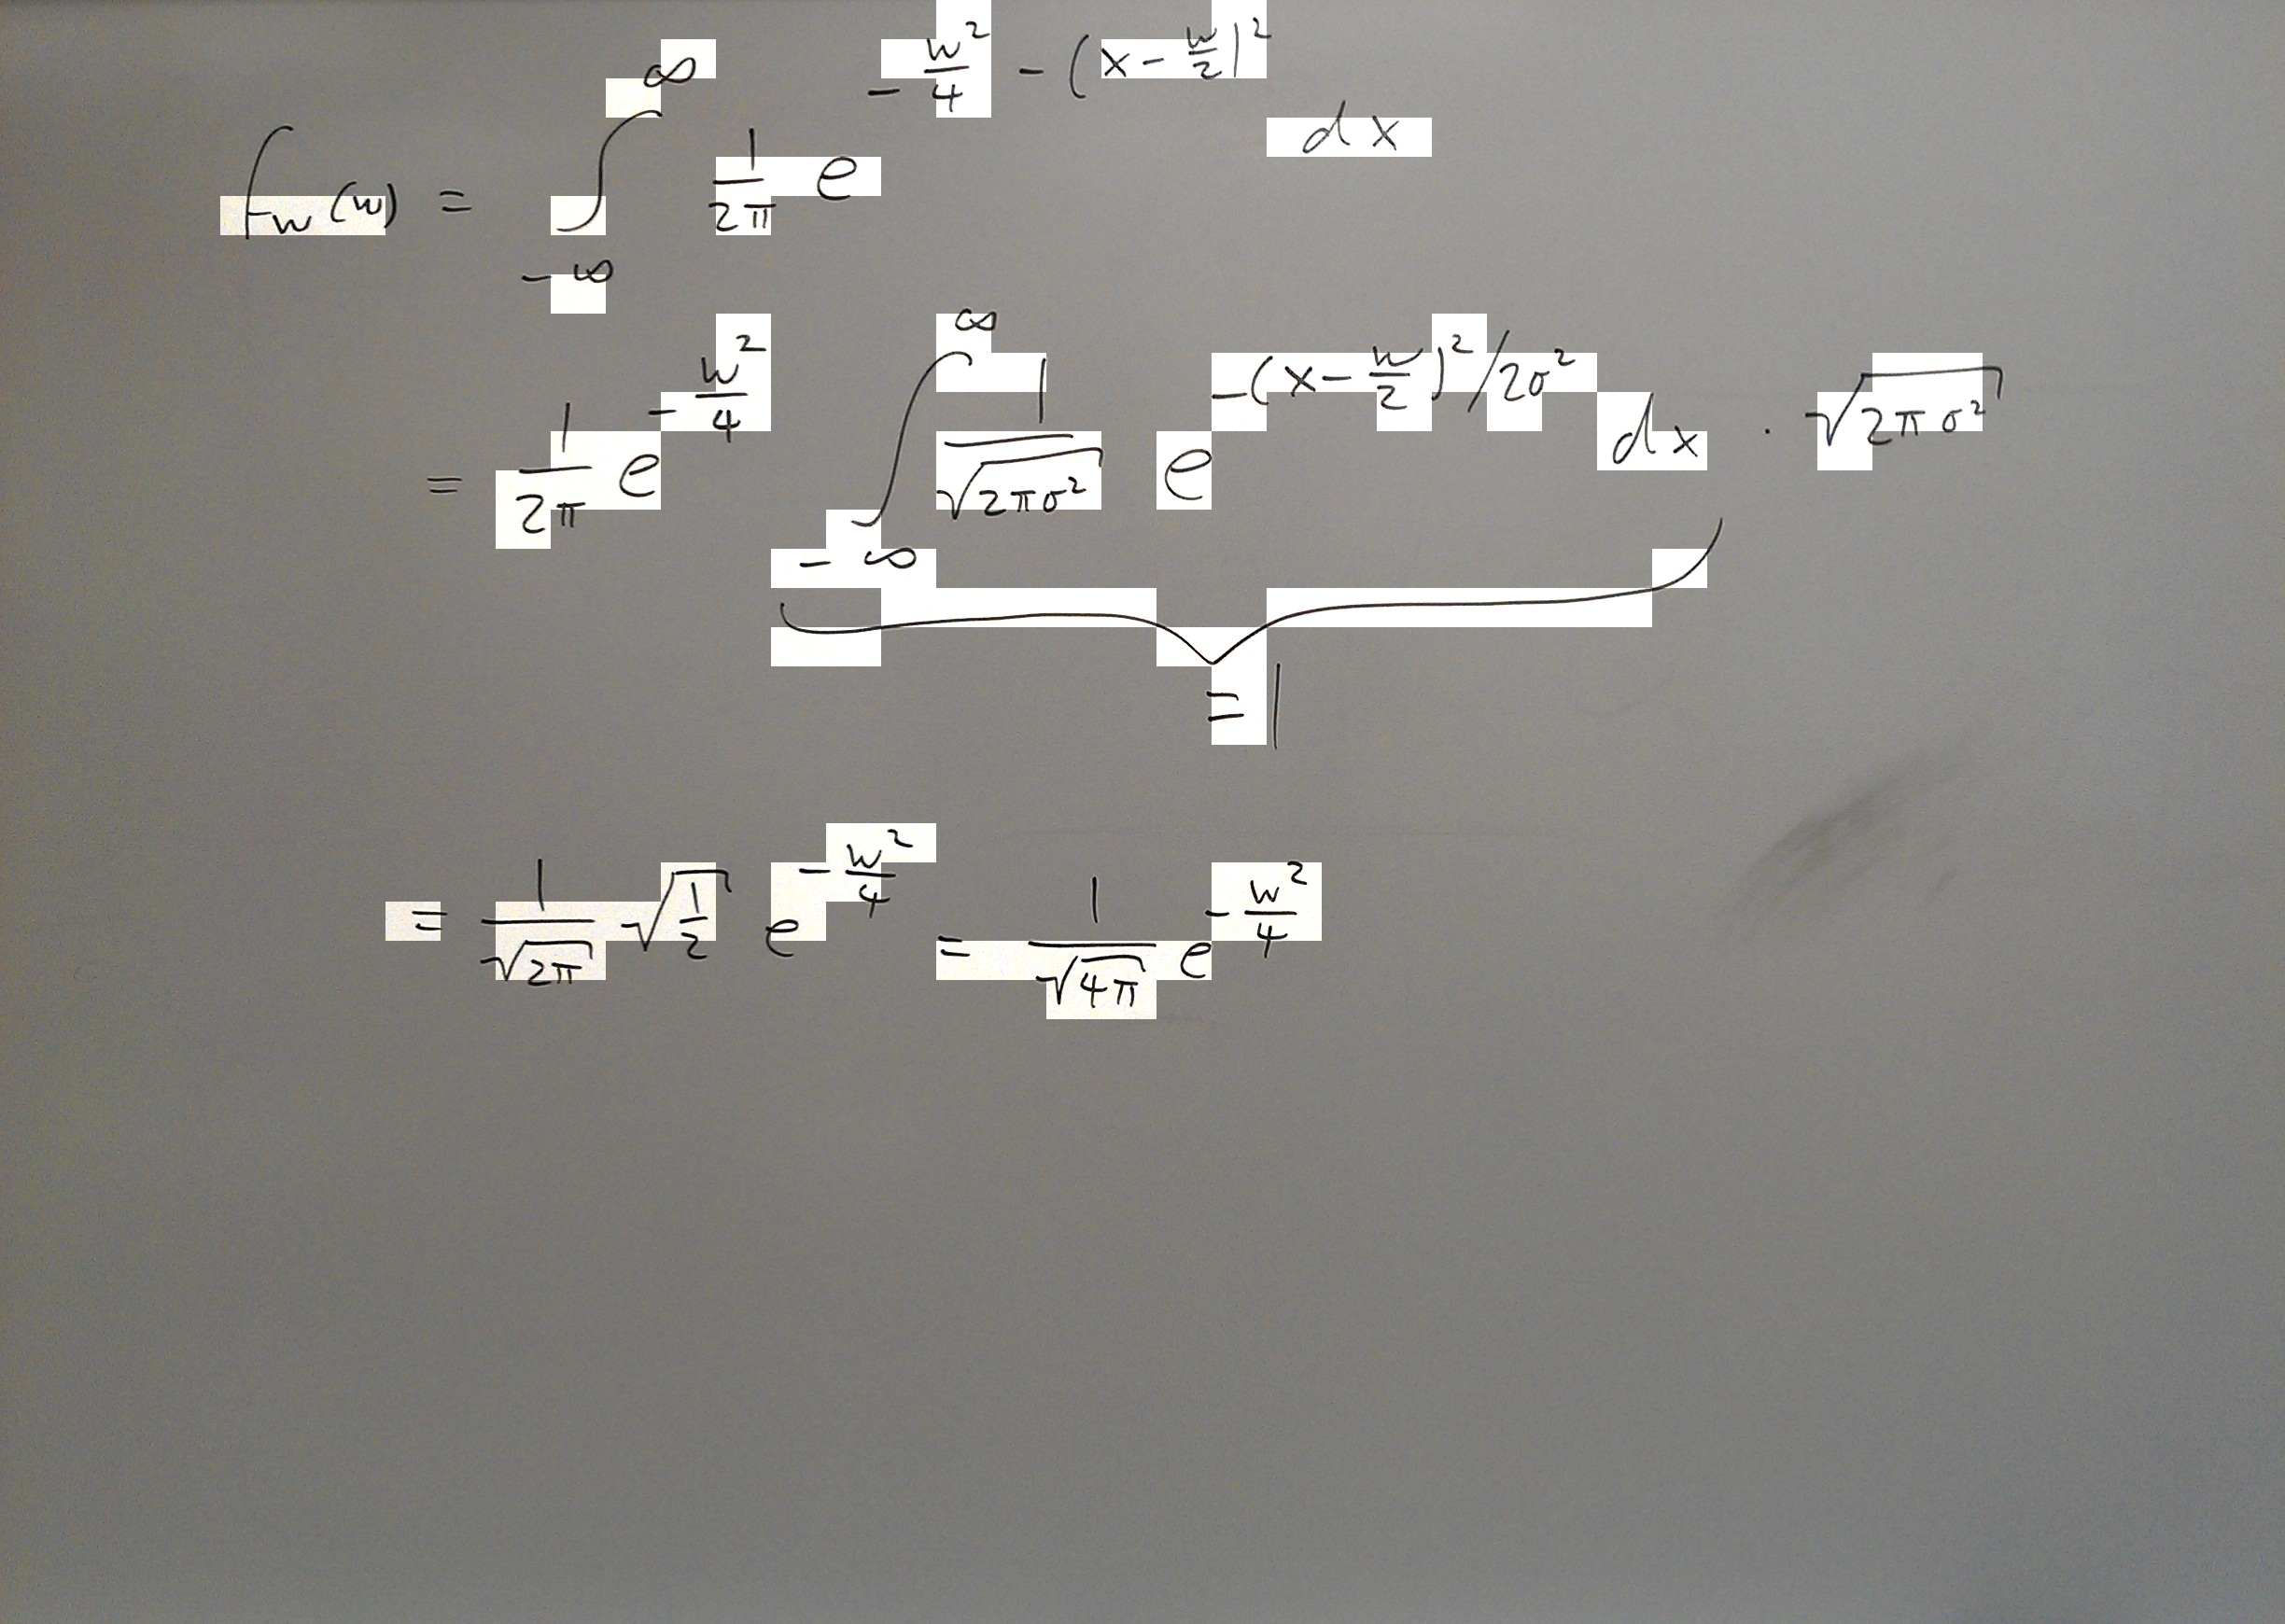
\includegraphics[scale=0.15]{images/cell_id_demo}
\caption{Image with stroke cells brightened}
\end{figure}

\begin{figure}[H]
\centering
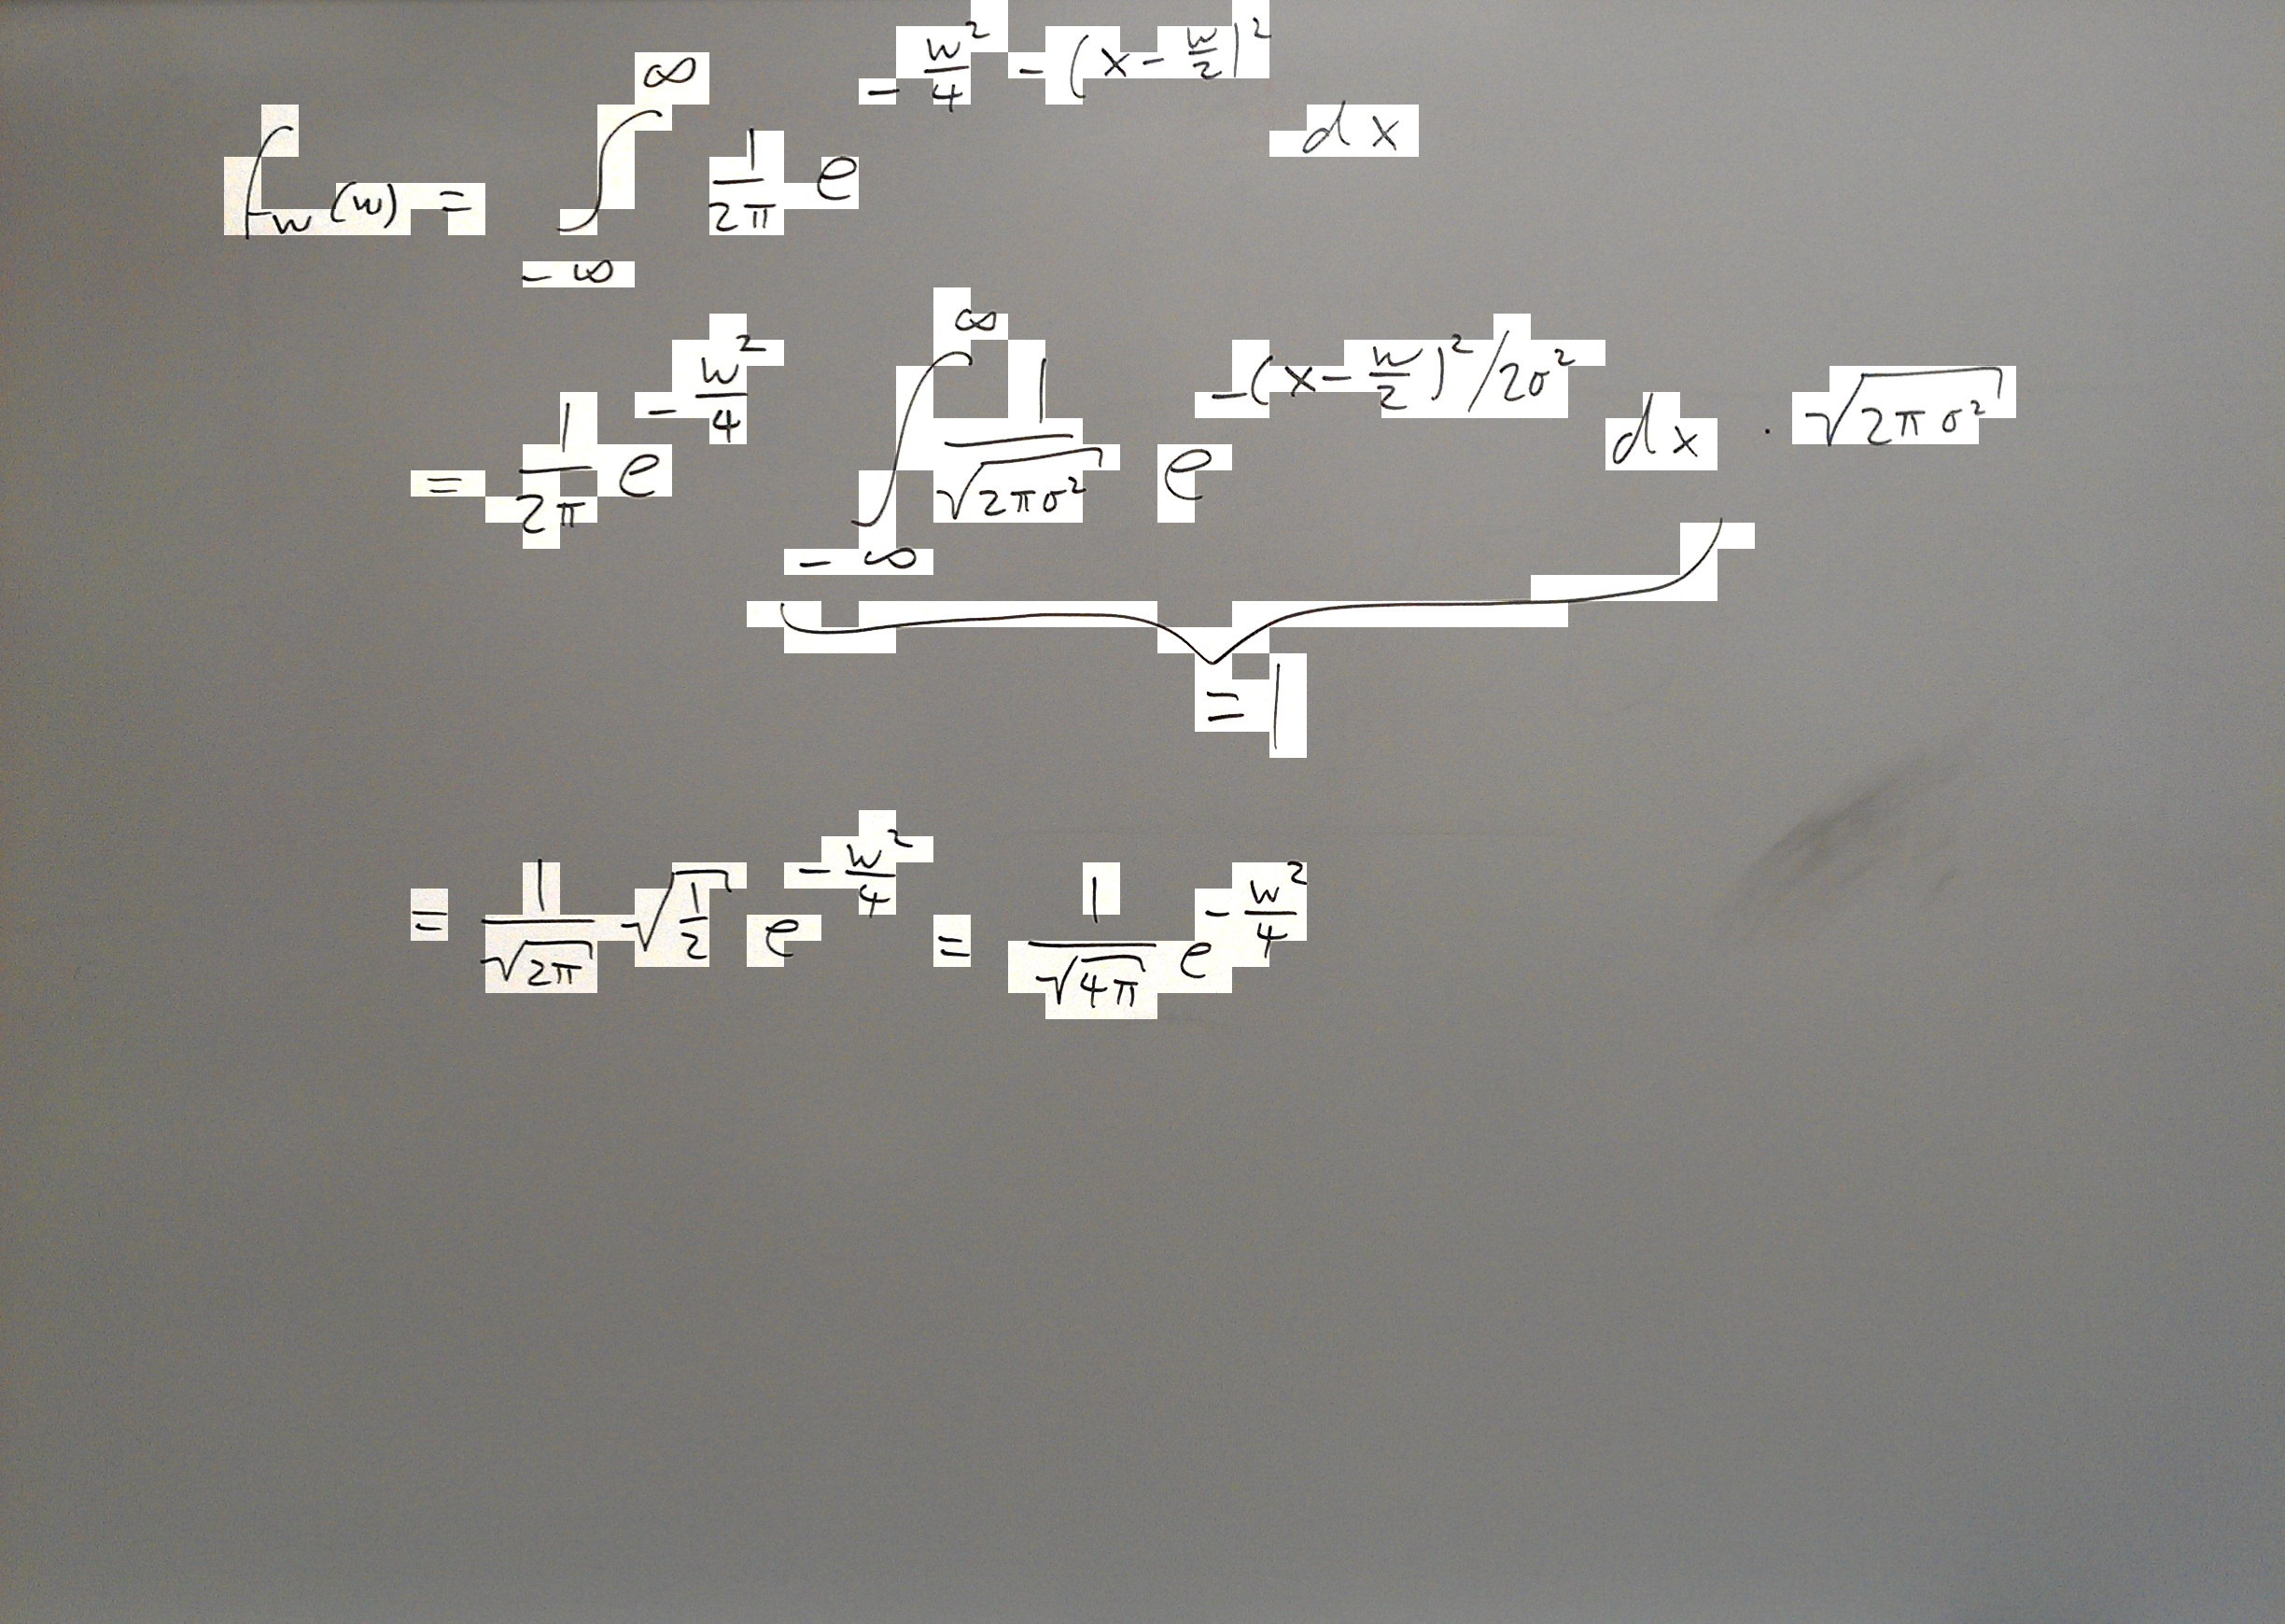
\includegraphics[scale=0.15]{images/cell_id_demo_61}
\caption{Same image, with smaller whiteboard standard deviation}
\end{figure}

\begin{figure}[H]
\centering
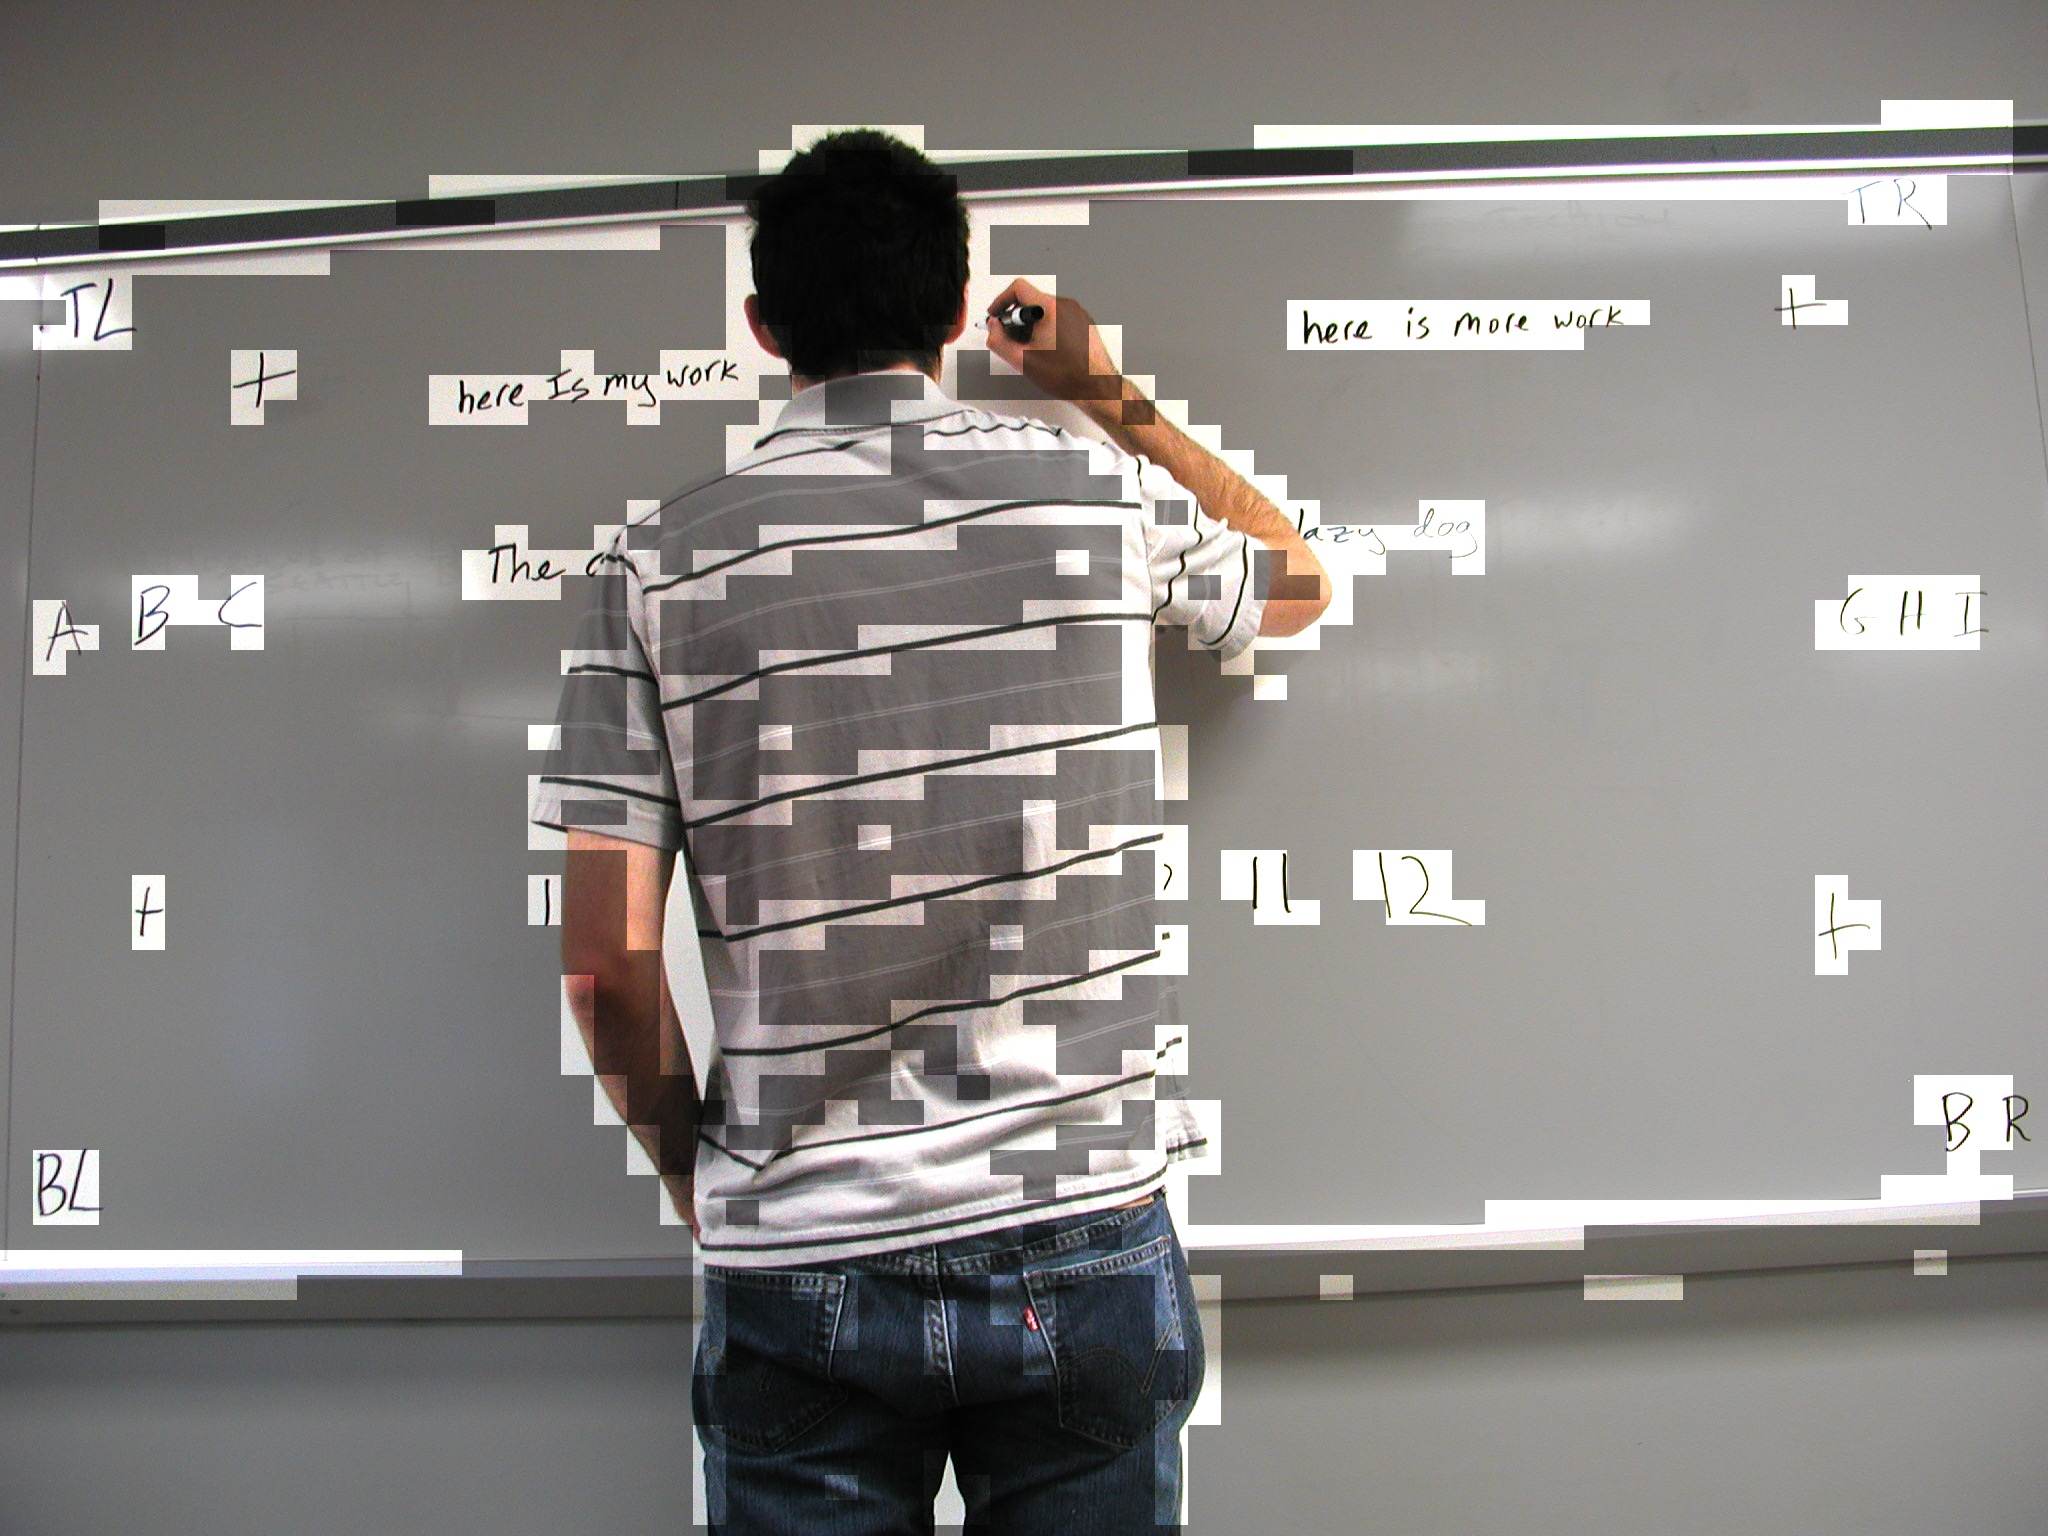
\includegraphics[scale=0.18]{images/cell_id_griffin}
\caption{Image with Griffin in front.  Note erroneously detected shirt stripes as stroke cells and no detection of foreground cells}
\end{figure}

Clearly, the stroke cell id works quite well, especially for a lower standard deviation.  Also, the stddev is not being correctly calculated;  I think it's because so far, I've been using single images.  What I need is images over time.  The script will need to be rewritten for that.  It also needs to be object-oriented.  This should also improve foreground cell detection.  


	%Sixteenth Entry
	\section{Dividing Images, Whiteboard Color Normalization (11/1/2012)}
	\subsection*{Dividing Images into Cells}
		I changed the cell division so that the cell images are put into a two-dimensional array.  Now, the image cells are located spatially in the same place as the images they represent in the picture.  This should make it easier to reference and operate on specific parts of the image.  I also needed a new way to demonstrate the changes that I can make on individual cells.  I used a two for loops (one for each dimension), and one uses modulo division to determine even or odd cells.
		
		\subsection*{Whiteboard Color Normalization}
		Now that we can break images into cells, we need to be able to extract the whiteboard color, and normalize the whiteboard color so that it is uniform across the entire board.  I started by attempting to follow the strategy laid out in Microsoft's paper.  Their method was to take the luminance of every cell image and apply a histogram to obtain the most common color value in each cell.  Then, create a cell with that color value and fill the new image with cells of the whiteboard colors.  A sample of the code I wrote is below:

\begin{verbatim}
for i in nsize:
    for j in nsize:
        lum[i][j] = cell_image[i][j].convert("L")
        hist[i][j] = lum[i][j].histogram()
        big[i][j] = max(hist[i][j])
        white[i][j] = hist[i][j].index(big[i][j])
        wb[i][j] = Image.new("L",(cell_width,cell_height),white[i][j])
        bkgd[i][j] = wb[i][j].convert("RGB")
        im_new.paste(bkgd[i][j], cell[i][j])
im_new.show()
\end{verbatim}

\begin{figure}[H]
\centering
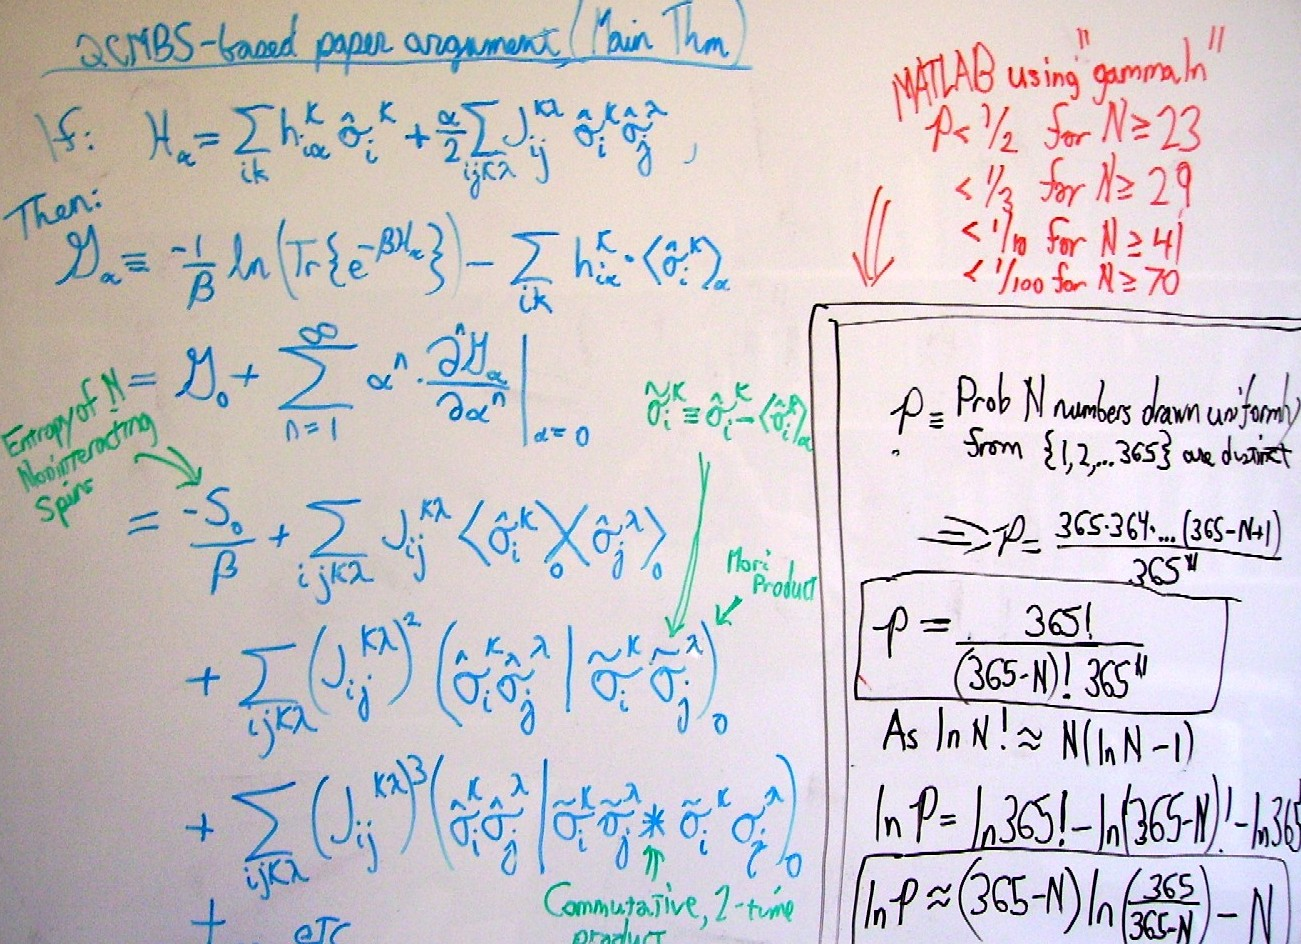
\includegraphics[scale=1]{images/whiteboard_cropped}
\caption{The whiteboard image seen in figure \ref{fig:whiteboard} (from 10/29 work log), cropped so that only the board content is displayed}
\label{fig:whiteboard_cropped}
\end{figure}

\begin{figure}[H]
\centering

\includegraphics[scale=0.25]{images/wb_crop_background_1}
\caption{A 21 by 21 cell image with the whiteboard color extracted}
\end{figure}

\begin{figure}[H]
\centering

\includegraphics[scale=0.25]{images/wb_crop_background_2}
\caption{A 41 by 41 cell image with the whiteboard color extracted}
\end{figure}

\begin{figure}[H]
\centering
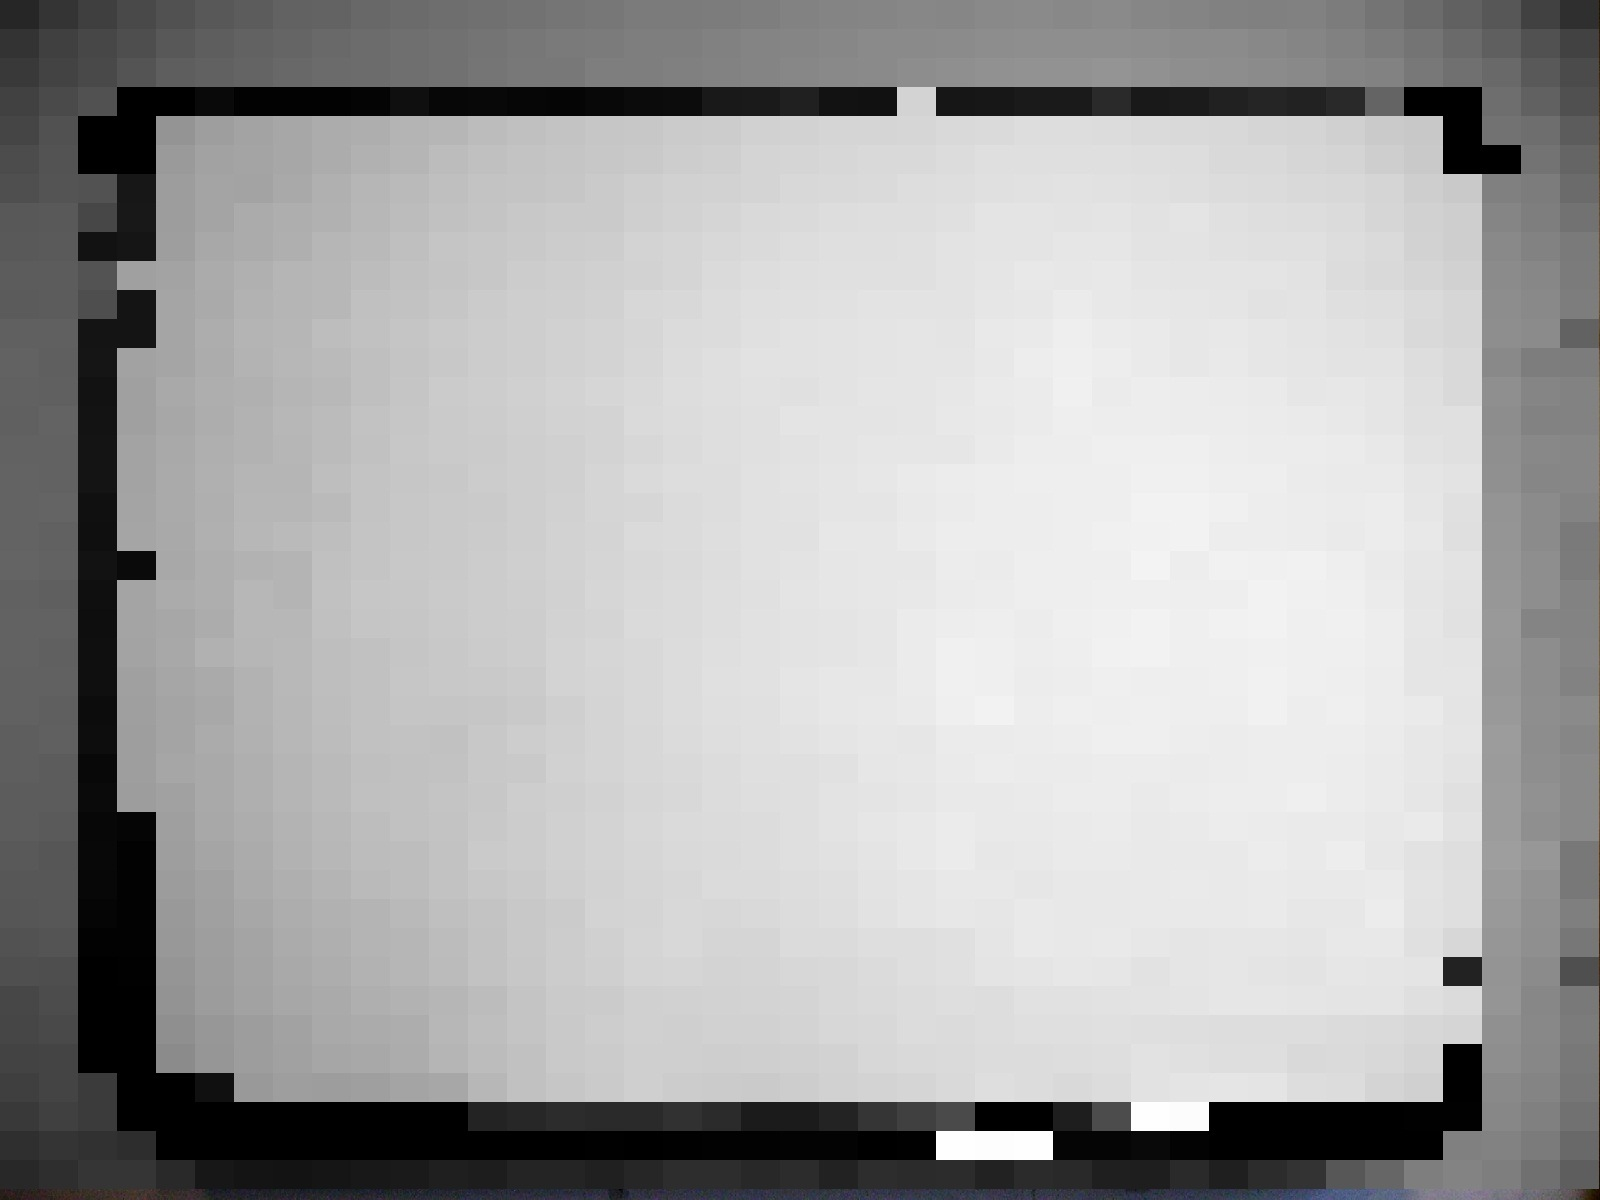
\includegraphics[scale=0.25]{images/wb_background}
\caption{The whiteboard image from figure \ref{fig:whiteboard}, processed by the code seen above.}
\end{figure}

This image demonstrates that the normalization of the cell images may be useful for more than just whiteboard color normalization.  The edges of the whiteboard are very defined, and may be useful for edge detection.

	%Fifteenth Entry
	\section{Post Panel 2, Dividing Images into Cells (10/29/2012)}
	Note:  I have not yet received a response from anyone involved with the Microsoft project.  If I don't hear back by this week's senior design meeting, I will talk to MST and/or Dr. Watkins about using their contacts.
		\subsection*{Post Panel 2}
	Our panel meeting went well - we updated everyone present on our progress, and received some good feedback about our plans going forward.  Bill from the CTDI group suggested that we look into Image Magic (related to J Magic) for image processing applications.  He said it works with Java or Python, so we will have to at least look at it.  
		\subsection*{Dividing Images into Cells}
	I was able to take an image and divide it into cells.  Right now, I can divide it arbitrarily into  cells, though in the final project we will choose the number of cells to be a size that is relevant to the size of content on the board.  \\
	To divide the image into cells, I wrote a script that divides the image width and height into $n$ segments, then goes through and creates $n^2$ cells from the image.  Each cell can then be individually modified.
	
\begin{verbatim}
import Image
import ImageEnhance

im = Image.open("whiteboard.jpg")
width=im.size[0]
height=im.size[1]
n=5
cell_width=width/n
cell_height=height/n
cell = (n**2)*[0]
cell_image = (n**2)*[0]
x=0

for i in range(0,n):
    for j in range(1,n+1):
        cell[x]= ((j-1)*cell_width, i*cell_height, j*cell_width, (i+1)*cell_height)
        cell_image[x] = im.crop(cell[x])
        x=x+1
\end{verbatim}
	
This code will divide an image into 25 cells.  To illustrate this, consider the image below.

\begin{figure}[H]
\centering
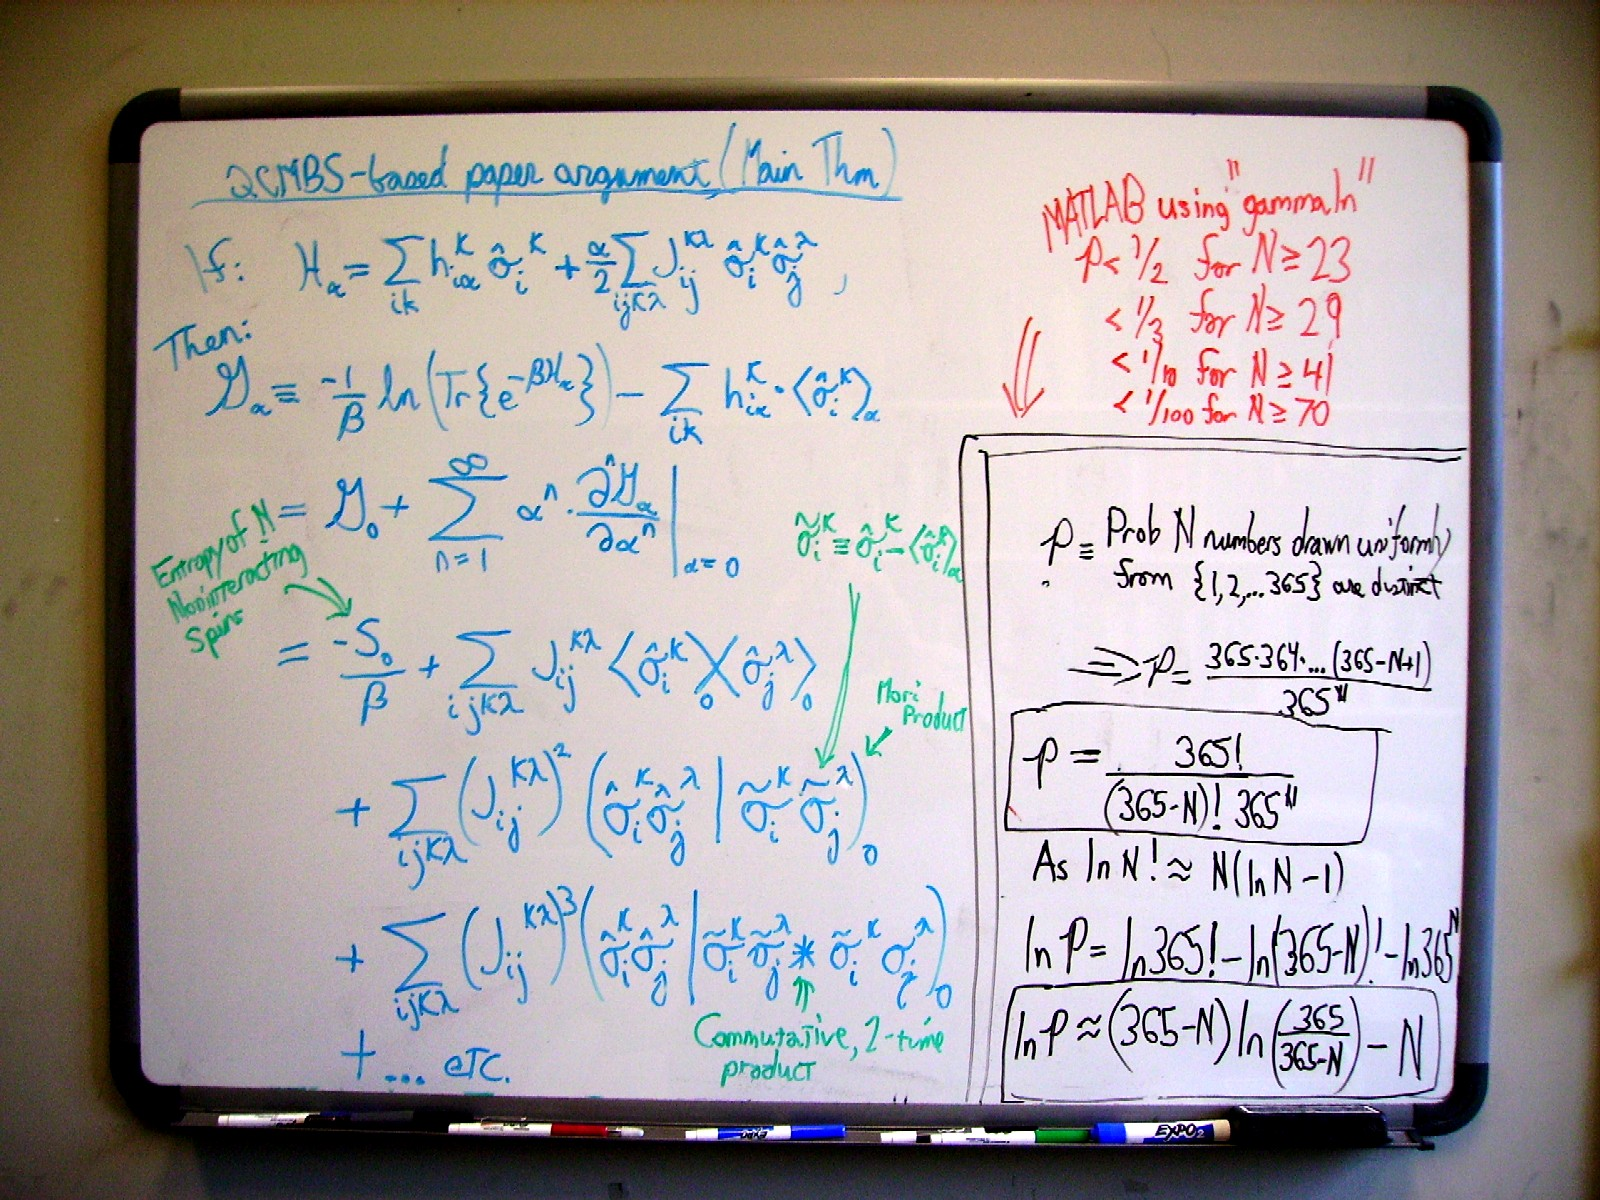
\includegraphics[scale=0.6]{images/whiteboard}
\caption{A typical whiteboard. Source: Google Images}
\label{fig:whiteboard}
\end{figure}	

Now, consider the image is divided into cells using the above process. If no operations are done on it, the image looks identical to the original.  Below is the same image, with a brightness filter applied to every other cell.

\begin{figure}[H]
\centering
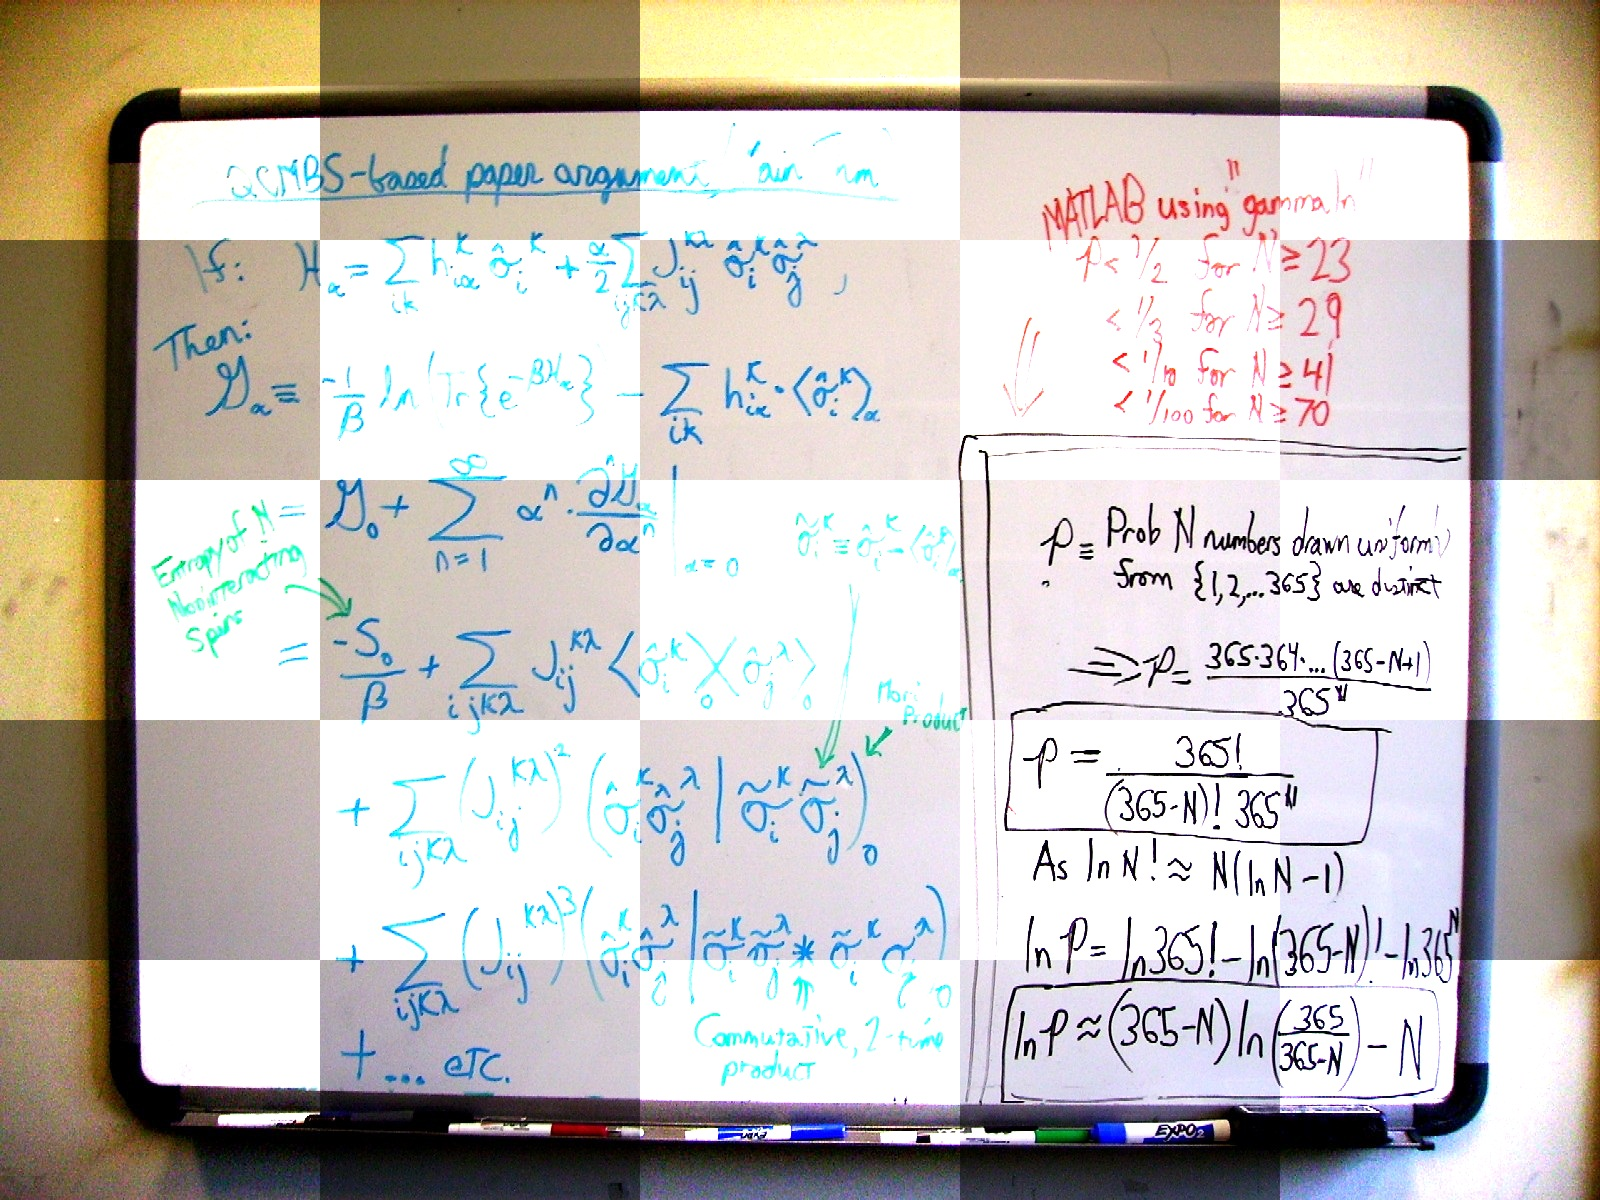
\includegraphics[scale=0.15]{images/cell_brightness_5}
\end{figure}	

The following code was used to create this image: 
\begin{verbatim}
checkered = range(0,n**2,2)

for i in checkered:
    temp = ImageEnhance.Brightness(cell_image[i])
    temp = temp.enhance(2.0)
    im.paste(temp, cell[i])
im.show()
\end{verbatim}

This can be scaled to any $n$ value, as seen below, but with a contrast filter.

\begin{figure}[H]
\centering
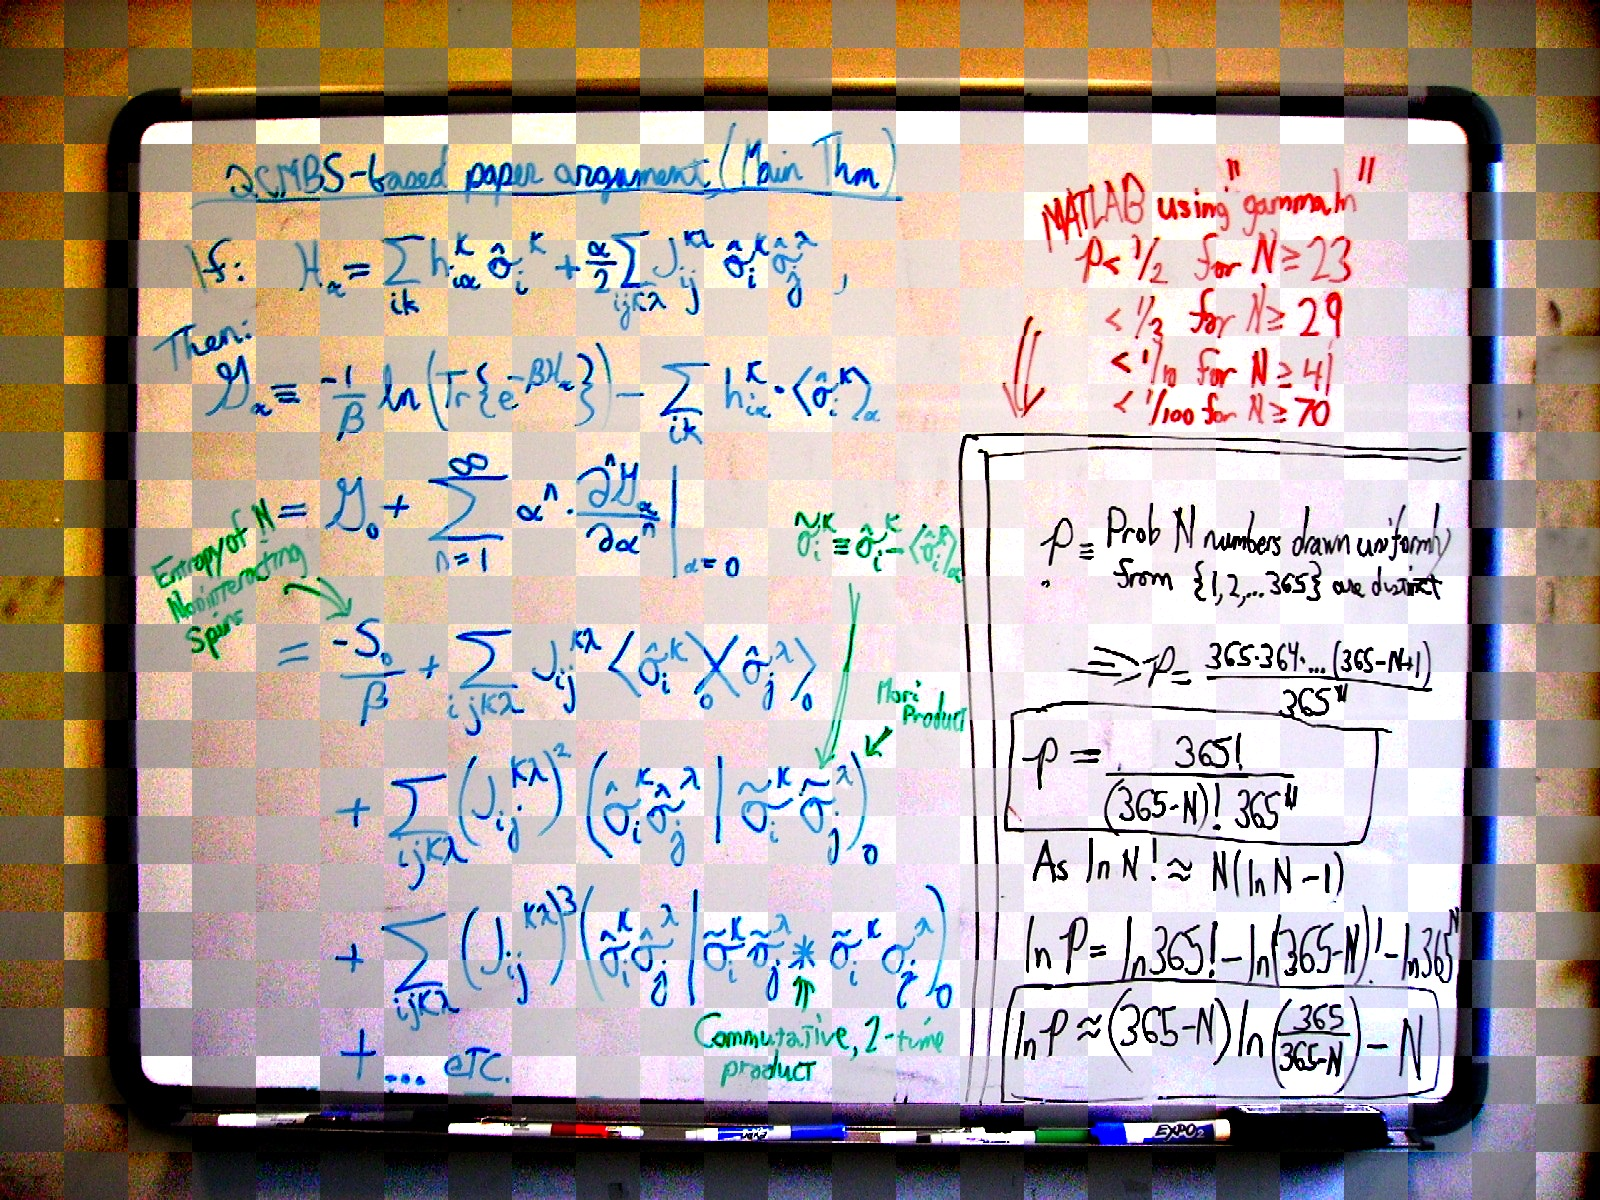
\includegraphics[scale=0.15]{images/cell_contrast_25}
\end{figure}


	%Fourteenth Entry
	\section{Gantt Chart, Preparation for Faculty Panel 2 (10/24/2012)}
		\subsection*{Gantt Chart}
	I finished the Gantt chart.  I ended up using an online Gantt chart program (\url{tomsplanner.com}).  It is easy to use and looks nice... the only disadvantage is that I can't export it without a paid membership.  For now I'm just screen-capturing it.  I plan on switching the chart to Microsoft Project in the future.
		\subsection*{Panel 2}
	The Gantt chart is ready to go, and I used the information from the chart to update our schedule document, which is essentially a narrowed-down text version of the Gantt chart.  
	
	%Thirteenth Entry
	\section{Microsoft, Gantt Chart, Learning Python (10/20/2012)}
		\subsection*{Contacting Microsoft}
	I sent an email to the three people listed on the WCS paper explaining to them what we are trying to accomplish, and asking if they could give us any help via access to parts of their work.  I am waiting for a response.
		\subsection*{Gantt chart}	
	I am in charge of making the Gantt chart for our group. I am looking into different free options for chart creation. I found something that templates a Gantt chart in Excel, but it doesn't look very good and I'm looking for something better.  As far as assigning tasks, we have talked about it as a group, so people are working on tasks that are most suited to their skills and interests.  Griffin is doing a lot of the work towards identifying a camera, and Phil and I are looking to start doing image processing.
		\subsection*{Python}
	I'm still working through lessons on Codecademy.  Mainly, they teach the syntax of Python: The importance of white space, math operations, loops, etc...  They have been helpful so far, but soon I'll just need to jump in to our task and learn the relevant parts as I go.  
	%Twelvth Entry
	\section{Risk Meeting, Tasks Going Forward (10/18/2012)}
		\subsection*{Meeting with Prof. Thompson}
	Today we met with Prof. Thompson about our risk analysis.  I think now we better understand what is expected of us going forward this semester.  We should focus more on proving that certain concepts will work, not necessarily implementing them as we will in our project.  For example, we should see how to do basic relevant image processing using libraries for Java, C++, Python, etc... and compare the processes.  
		\subsection*{Individual tasks going forward}	
	Going forward, I first need to contact Microsoft Research to try and acquire the source code from the WCS.  This will hopefully simplify the image processing aspect of our project, since we could use their code as a guideline for our own, or possibly even use entire chunks of their code in our implementation. \\
	\indent Currently, we need to make a Gantt chart for our semester schedule.  Then I will look into various aspects of image processing and come up with demos to demonstrate progress.  Currently I'm trying to learn Python from \url{codecademy.com}, since background research suggested that it may be the easiest language for the tasks we're trying to complete.
	
	
	%Eleventh Entry
	\section{Risk Analysis (10/16/2012)}
		\subsection*{Risk}	
	In class last week, we worked on risk analysis and planning. Here is the list I came up with of possible risks and their level of risk:
	\begin{itemize} \itemsep -2pt
	\item \textbf{HIGH -} What language/framework to use?
	\item \textbf{HIGH -} Specific image processing libraries?
	\item \textbf{HIGH -} What camera? Android compatible? (Nikon, Samsung)?
	\item \textbf{HIGH -} How to interface camera with computer?
	\item \textbf{HIGH -} Wireless syncing?
	\item \textbf{MEDIUM -} Database for images? How to add to it from camera
	\item \textbf{LOW -} Can students access photos directly?
	\item \textbf{LOW -} How to distribute images? Dropbox? Netspace? Email?
	\item \textbf{LOW -} Does the camera need a stand?
	\item \textbf{MEDIUM -} Adjusting for capture angle (second edition)
	\item \textbf{MEDIUM -} Automatic recognition of board area
	\item \textbf{MEDIUM -} Key frames: only right before erase (like WCS)?
	\item \textbf{LOW -} Manual frame capture option
	\item \textbf{MEDIUM -} Filters for students w/ learning disorders
	\end{itemize}		
	
	Possible Demos: 
	\begin{itemize}
	\item Image noise removal 
	\item Identify person in image
	\item Remove person/replace with another image
	\item Rapid automatic image capture
	\end{itemize}
	
		\subsection*{Idea}
	During class I thought of a possible idea for filtering images on the whiteboard by color and content.  All board content could be displayed as a 3D matrix, as in the Microsoft system.  However, we could take it a step further and filter by color as well, since professors will sometimes write groups of related information in the same color. This is definitely true for civil engineering professors, based on notes provided to us by our client. \\
\begin{figure}[H]
\centering
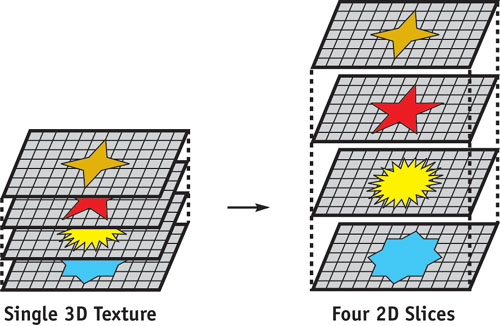
\includegraphics[scale=0.4]{images/3D_matrix}
\caption{Idea similar to this image}
\end{figure}	
	\indent The board could be represented by a matrix of cell images, with the width and height representing the board dimensions, and the depth ``in and out'' of the board representing different groupings.  For instance, the whiteboard cells could all be in the same plane of the matrix, while any foreground (undesirable) objects could be in another plane. The rest of the board content could be in other planes, sorted by color. So for instance, all black writing would be in a particular plane, while blue writing would be in another.  By default, the processed image would remove foreground objects and display whiteboard and all writing, but the user could manually choose to only see, for instance, writing and drawings in red, or everything except green.  This feature could be useful to students with learning disabilities, since it would simplify the image and group relevant information together.




	% Tenth Entry
	\section{Final Version of Background Document (10/12/2012)}
	We uploaded our final version of the Background document to our git repo tonight.  (Speaking of that, our ProPANE site now links to the git hub for all documents, so we don't have to worry about changing that on the site every time.)  I added in all my research about signal processing, including code libraries, basic image processing concepts, and various image processing techniques that can be utilized.  We figured out some hitches with git so that we could successfully merge our separate changes into one document.  \\ \\

I did some more research into the Nikon COOLPIX s800c camera.  It is the only Android-powered camera currently on the market.  I found that it is theoretically available in-store at the Target in Selinsgrove, so I plan on driving down there some time soon to check it out in person.  


	% Ninth Entry	
	\section{Work on Background Document, Use of git for Version Control (10/9/2012)}
	\subsection*{Background Research}
	I am doing basic research on the field of signal processing, and specifically image processing.  A lot of it is simply looking for reliable sources to cite and take information from.  As far as code libraries go, there are A LOT of different image processing libraries out there for a plethora of different platforms.  I am trying to mainly look at ones that are either free, or that Bucknell has access to (MATLAB and Mathematica).  Speaking of those two, I found a great chart comparing them: \url{http://en.wikipedia.org/wiki/Comparison_of_image_processing_software} 

	\subsection*{git}
	We decided to use git for version control.  I made an account on github and cloned our repository to my system.  Now, we can all access the same files at all times. This is especially helpful for compiling LaTeX documents, since embedded images must be included in the directory, and any of us might add those.  





	% Eighth Entry
	\section{Third Client Meeting (10/5/2012)}
	We met with our clients and Prof. Thompson following our faculty panel.  We discussed some ideas that will help our project, and Prof. Thompson gave us some important feedback and suggestions.

\begin{itemize}
\item We need to touch on non-performance specs in our tech specifications: 
	\begin{itemize} \itemsep -2pt
	\item Wired vs. Wi-Fi
	\item skewing
	\item color
	\item saturation
	\item flash
	\end{itemize}
\item We should email Dr. Midkiff about the setup of classrooms on campus, especially the new Academic West area.
\item Include option for a manual key frame capture
\end{itemize}
	
\textbf{Information for our background document: }
\begin{itemize}
\item Take a hierarchical approach 
\item Provide reasons for researching products
	\begin{itemize} \itemsep -2pt
	\item Why do they benefit us 
	\item Why are they grouped as such in document?
	\end{itemize}
\item Explain why the WCS is so important
\item Include research on signal processing
	\begin{itemize} \itemsep -2pt
	\item Look for code libraries that perform image processing
	\item General Concepts and points of interest regarding signal processing
	\end{itemize}
\item Look into applicable learning disabilities - what students need and why
\end{itemize}
	% Seventh Entry
	\section{Panel Feedback, Continued Research (9/30/2012)}
	Following the first faculty panel, we received some feedback that we will follow up with.
\begin{itemize}
\item We should contact Microsoft Research about getting any of the code used for their Whiteboard Capture System
\item Our capture system will need a capture device (obviously).  We should look into a smart camera by Nikon that runs Android, as well as a Samsung Galaxy camera that we previously found.  
\item We should assume that for our system, the distance from the board is constant.  We need to determine what that should be.  
\item We need information about the desired resolution of our camera.  
\end{itemize}

	% Sixth Entry
	\section{First Panel, Continued Research (9/27/2012)}
	I created an agenda for our first panel, and I got the specs and background documents together so each attendee could have one.  \\ \\
I am continuing background research into related technologies.  Currently, I'm looking at ReBoard, a whiteboard system who's greatest strength is its ability to sort captured data by a lot of different metadata. Info can be found \href{http://arxiv.org/ftp/arxiv/papers/0911/0911.0039.pdf}{here}.

	% Fifth Entry 
	\section{Additional Information on Microsoft Whiteboard Capture System (9/21/2012)}
	The research on the Microsoft Whiteboard Capture System (WCS) is done, and will be included in our Background and Research document.  I talked in detail about that system's method of capturing data and processing it.  The paper gave many mathematical examples on how they accomplished certain steps of their system, but I did not include them in the research document, so I will discuss them here.
	\subsection*{Clustering Cell Images Over Time}
	As the meeting progresses, the WCS groups cell images from the same cell together if it determines that they don't change over a period of time.  This is done using a modified Normalized Cross-Correlation algorithm to determine if two cells are the same or different.  It is demonstrated here for one color, but applies to all RGB components.  \\
Consider two cell images $I$ and $I'$.  Let $\bar{I}$ and $\bar{I'}$ be their mean colors and $\sigma$ and $\sigma'$ be their standard deviations.  The normalized cross-correlation score is given by \[ c={1 \over N \sigma \sigma'} \sum (I_i - \bar{I})(I_i' - \bar{I'}) \]
where the summation is over every pixel $i$ and $N$ is the total number of pixels.  The score ranges from -1, for two images not similar at all, to 1, for two identical images.  Since the score is computed after the subtraction of the mean color, it may still give a high value even if two images have very different mean colors.  So a different test is performed on the mean color difference, based on the Mahalanobis distance \href{http://en.wikipedia.org/wiki/Mahalanobis_distance}{(info)}.  The distance is given by 
\[ d={|\bar{I}-\bar{I'}| \over (\sigma + \sigma')} \]
Two cells are considered to be identical and are grouped together if and only if $d<T_d$ and $c>T_c$.  In the WCS implementation, $T_d=2$ and $T_c=0.707$.
	\subsection*{Classifying Cells}
It must be determined whether a cell image is a whiteboard, stroke, or foreground object.  The determination is based on whether or not a cell's color distribution is the same, similar, or very different from that of the whiteboard.  As above, the Mahalanobis distance is used, and calculations are for one component of RGB.  \\
\indent Let $\bar{I}_w$ be the whiteboard color and $\sigma_w$ be the standard deviation (small since a whiteboard cell is basically uniform).  Then let $\bar{I}$ and $\sigma$ be the mean and standard deviation of the current cell image.  The cell image is classified as a whiteboard cell if and only if \[ {|\bar{I} - \bar{I}_w| \over (\sigma + \sigma_w)}<T_w \quad \textrm{ and } \quad  {\sigma \over \sigma_w }< T_\sigma \] 
and as a stroke cell if and only if
\[{|\bar{I}-\bar{I}_w| \over (\sigma + \sigma_w)}<T_w \quad \textrm{ and } \quad {\sigma \over \sigma_w} \geq T_\sigma \] 
Otherwise, it's classified as a foreground object cell.  In the WCS implementation, $T_w=2$ and $T_\sigma=2$.
	\subsection*{Key frame color balance}
The background must be uniformly color-balanced and the color saturation of the pen strokes must be increased.  The previously-calculated whiteboard color, $\bar{I}_w$ is used to scale the color of each pixel in the cell. \[ I_{out} = \textrm{min} (255, {I_{in} \over I_w} \cdot 255) \]
Image noise is reduced by remapping the value of each color channel of each pixel in the key frames according to an S-shaped curve.

	% Fourth Entry
	\section{Review of Second Client Meeting, Background Research (9/17/2012)}

		\subsection*{9/13 Meeting Review}
Met with Dr. Midkiff and Dr. Gabauer regarding our technical specifications.  They made a couple of suggestions for modification of our specs (bold numbers refer to tech spec section numbers):
\begin{itemize}
\item \textbf{3.1.2} Setup time can be longer than our suggested 5 minutes if it's a one time process (or once daily) and the settings can be saved for multiple uses. Active vs. passive setup time is important.
\item \textbf{3.3.2} Key frames should be time-stamped
\item \textbf{6.2.2} User should be able to select other frames as ``key frames'' if he/she is not happy with the automatically chosen frames
\item \textbf{7.1} Transfer from professor to student \textbf{must} be easy to use.  Ideas include email or a dropbox feature. \\  
\indent Notes must be delivered to students within 24 hours.  Therefore, all captured data should be in the hands of the professor well before then. \newline
\hspace{0.1in} End-users (students) should be able to edit images as well. Suggested features include zoom in/out, viewing of frames preceding and following key frames.  \sl{These may be included in Version 2}
\end{itemize}
		\subsection*{Continuing research}
I am finalizing a section of research on the Microsoft Whiteboard Capture System mentioned in the work log on 9/5.  I am also starting research on another system, the ReBoard, as mentioned \href{http://www.fxpal.com/publications/FXPAL-PR-10-546.pdf}{here} and \href{http://www.fxpal.com/?p=reboard}{here}.  
		

	% Third Entry
	\section{Tech Specs, Second Meeting, Website Design (9/11/2012)}

		\subsection*{Technical Specification Document}
		Worked with Phil on the first draft of the Specification and Testing document \href{https://docs.google.com/viewer?a=v&pid=sites&srcid=ZGVmYXVsdGRvbWFpbnxidXByb3BhbmV8Z3g6NjhkOWVjMjIyZjY3ZTM4ZA}{(link)}.  We outlined general areas that we need to have specifications for, including hardware, software, interface, and legal requirements.  We are not far enough along with research to begin making specific declarations regarding most technical areas, but we outlined what we will need to define in the future.  Additional details regarding specs will also be outlined in our upcoming meeting with our clients.

		\subsection*{Second Client Meeting}
		I arranged a meeting with Dr. Gabauer and Dr. Midkiff for 3 pm on 9/13/12 \href{https://docs.google.com/viewer?a=v&pid=sites&srcid=ZGVmYXVsdGRvbWFpbnxidXByb3BhbmV8Z3g6NDMwMGY4NTlmYWQ2NjUx}{(agenda here)}.  I arranged a conference room in Dana through Judy of the EE department.  We are meeting about the technical specifications of our project.  Dr. Midkiff will provide crucial input on the legal requirements we face due to designing a device for special needs students.  Dr. Gabaur's input will help us better understand the scope of the design and whiteboard capture process. The meeting will also help us prioritize the features of the first version of the product.

		\subsection*{ProPANE Site Changes}
		I made one small change to the website.  The homepage was extremely empty (prior to the project description being there) so I designed and added a graphic to fill space, while also helping viewers to understand our project at such an early stage.  It attracts the reader's attention with appropriately-colored text, it explains the ProPANE acronym, and it includes our logo.  This graphic is seen below.

\begin{figure}[H]
\centering
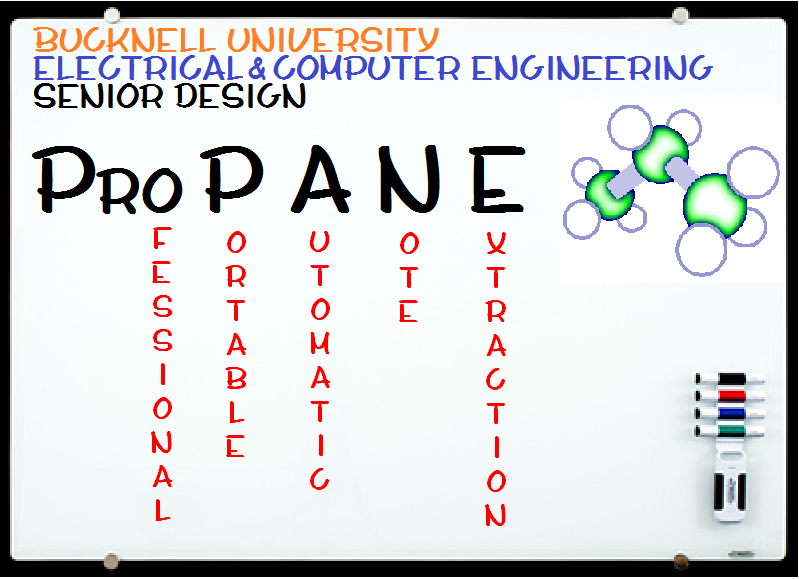
\includegraphics[scale=0.36]{images/propane_whiteboard}
\caption{Homepage image}
\end{figure}
 

	% Second Entry
	\section{Logo Design, Research on Background and Competition  (09/05/2012)}

		\subsection*{Logo Design}
		Worked on the ProPANE logo.  Tried different color schemes ranging anywhere from black and white, orange and blue (Bucknell) and black and gold.  Design was done in Adobe Photoshop and MS Paint.

\begin{figure}[H]
\begin{minipage}[b]{0.45\linewidth}
\centering
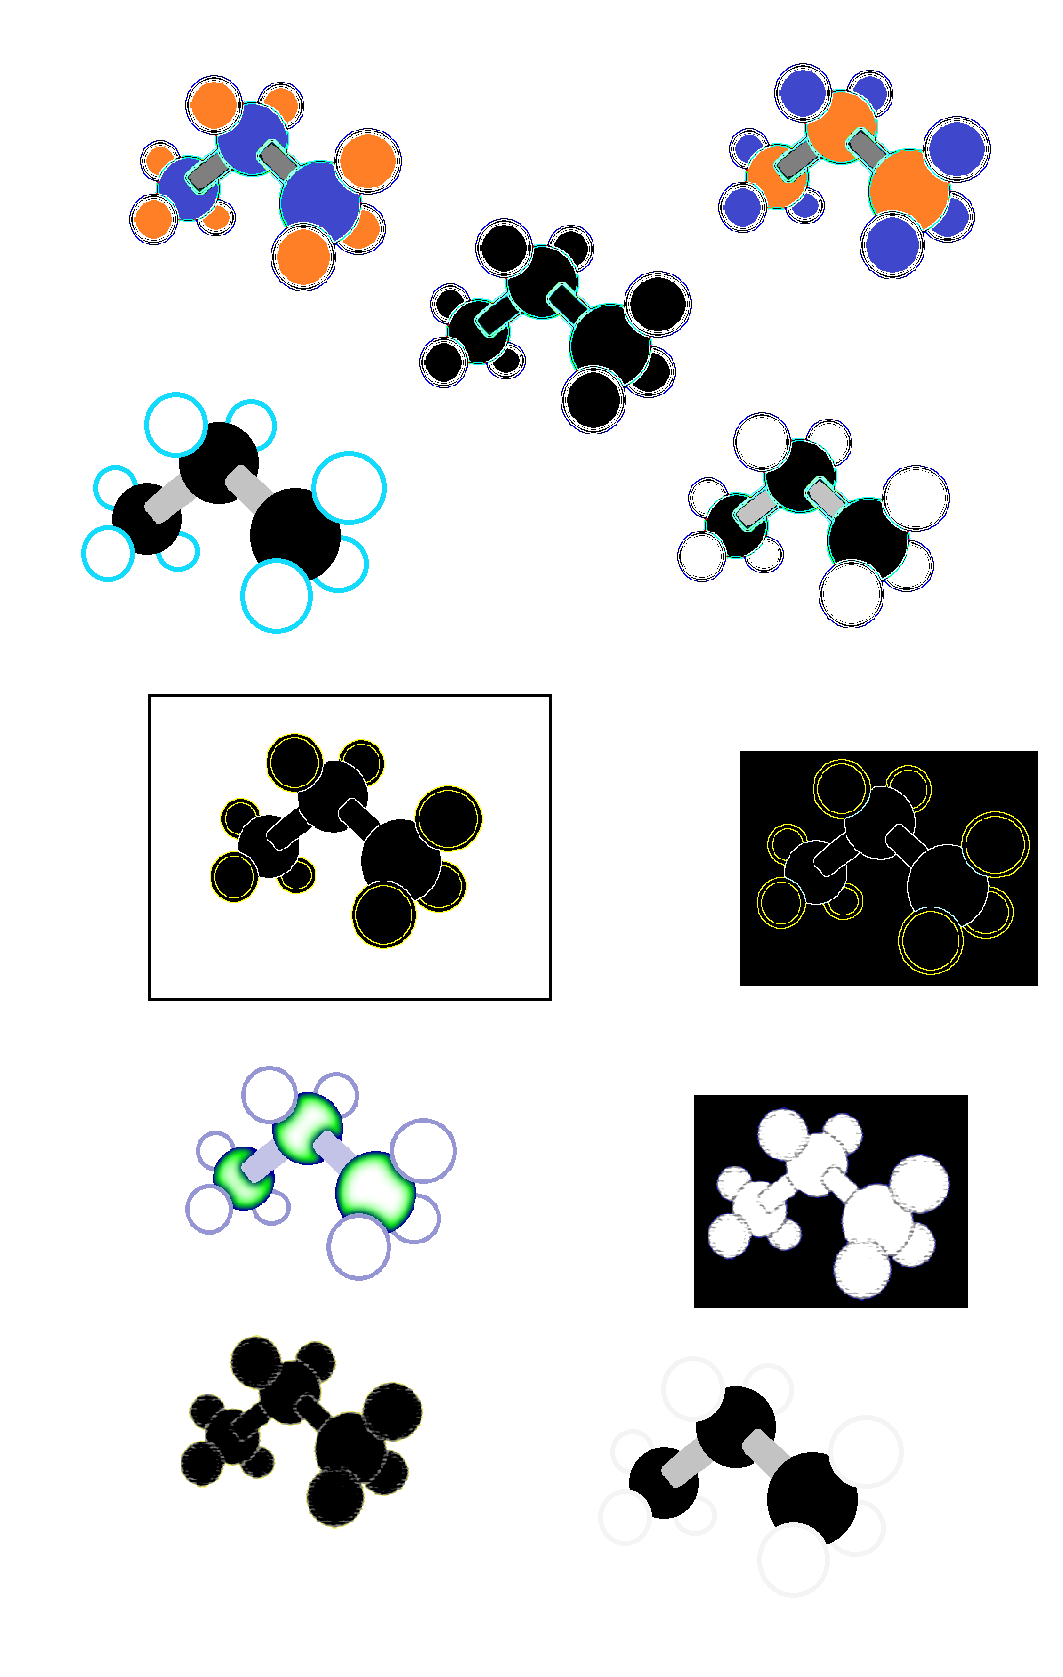
\includegraphics[scale=0.22]{images/logo_options}
\caption{Preliminary logo designs}
\end{minipage}
\begin{minipage}[b]{0.45\linewidth}
\centering
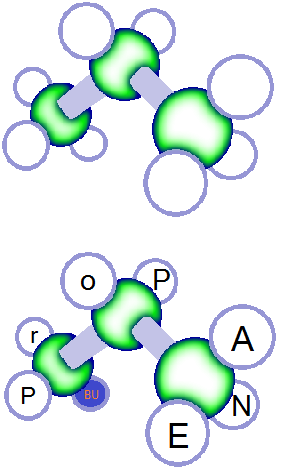
\includegraphics[scale=0.7]{images/ProPANE_final_logos}
\caption{Current ProPANE logos}
\end{minipage}
\end{figure}

Eventually the group settled on the current logos above, because they are easy on the eyes yet they still stand out.  \\

		\subsection*{Background Research}
			We began researching the different existing technologies that meet standards similar to that of our project.  One in particular seemed very similar to the design we are aiming for: a research project by Microsoft, their Whiteboard Capture System \href{ftp://ftp.research.microsoft.com/pub/tr/tr-2002-89.pdf}{(link)}.  I am in charge of analyzing it for inclusion in our Project Background and Research document.  

The Whiteboard Capture System is portable, works on any whiteboard, and provides a method of data distribution, all of which are desirable for our system.  However, it has some shortcomings (does not work on blackboards) and possible excess features (audio recording and playback).  Full  analysis will be included in the final document.    \\
			
			
			
	
	% First Entry
	\section{First Group Meeting and General Group Information  (08/31/2012)}
		
		Talked about the Initial Group Tasks.  Came up with a name, logo, and document template.  Discussed general tech specs and background information.    
		
		\subsection*{Technical Specifications}
			Our end design must be a portable system which captures notes written on a chalkboard or whiteboard, and distributes the information for later use.  We are looking into similar products which are currently on the market for background info and implementation ideas.  Dr. Midkiff plans to use our system to aid students with disabilities, so extra attention must be paid to ease of use and clarity of the final deliverable product.      \\
		
		\subsection*{Team Name and Logo}
			We wated to come up with an acronym that was both relevant to our project in some way, and also easy to say. We settled on the name BU ProPANE, which stands for \textbf{Pro}fessional \textbf{P}ortable \textbf{A}utomatic \textbf{N}ote  \textbf{E}xtraction.  We liked the idea of an already well-known word for the name, and we decided to design a logo with the same theme.  I am currently working with an image of a propane molecule to design a logo for BU ProPANE.    \\
			
		\subsection*{Document Template}
			We are using \LaTeX to format our documents and deliverables.  It was chosen because it takes care of formatting for us.   \\
			

\end{document}